\documentclass[10pt]{article}
\usepackage[margin=1in]{geometry}
\usepackage[utf8]{inputenc}
\usepackage{multicol}
\setlength{\columnsep}{1mm}
\usepackage{amsfonts}
\usepackage{booktabs}
\usepackage{siunitx}
\usepackage[authoryear,round]{natbib}
\usepackage{float}
\usepackage[font={small}]{caption}
\usepackage[labelfont=bf]{caption}
\usepackage{lineno}
\usepackage{amsmath,amssymb,setspace,fancyhdr,geometry,url,color}
\usepackage{subfigure,graphicx,caption}
\usepackage{lscape,amsthm}
\usepackage{blindtext}
\usepackage{hhline}
\usepackage{arydshln}
\usepackage{verbatim}
\usepackage{dblfloatfix}
\usepackage{multirow}
\usepackage{graphicx}
\usepackage{xr}
\externaldocument{../PhaseIIPaper/main}
%\biboptions{authoryear, comma}
%%%%%%%%%%%%%%%%%%%%%%%%%%%%%%%%%%%%%%%%%%%%%%%%%%%%%%%%%%%%%%%%%%%%%%%%%
%%%%%%%%%%%%%%%%%%%%%%%%%%%%%%%%%%%%%%%%%%%%%%%%%%%%%%%%%%%%%%%%%%%%%%%%%%
\begin{document}
\centering{\bf {\large Supplemental Material} \\
{\Large The GGCMI Phase II experiment: global gridded crop model simulations under uniform changes in CO$_2$, temperature, water, and nitrogen levels (protocol version 1.0)}}\\

\vspace{3mm}

\centering{James Franke$^{1, 2}$, 
Christoph M\"{u}ller$^3$, 
Joshua Elliott$^{2, 4}$, 
Alexander Ruane$^5$, 
Abigail Snyder$^6$,\\ 
Jonas J\"{a}germeyr$^{3, 2, 4, 5}$, 
Juraj Balkovic$^{7, 8}$, 
Philippe Ciais$^{9, 10}$, 
Marie Dury$^{11}$, 
Pete Falloon$^{12}$,\\ 
Christian Folberth$^7$, 
Louis Fran{\c{c}}ois$^{11}$, 
Tobias Hank$^{13}$, 
Munir Hoffmann$^{14,23}$, 
Cesar Izaurralde$^{15, 16}$,\\ 
Ingrid Jacquemin$^11$, 
Curtis Jones$^{15}$, 
Nikolay Khabarov$^7$, 
Marian Koch$^{14}$, 
Michelle Li$^{2, 17}$, 
Wenfeng Liu$^{18, 9}$,\\ 
Stefan Olin$^{19}$, 
Meridel Phillips$^{5, 20}$, 
Thomas Pugh$^{21, 22}$, 
Ashwan Reddy$^{15}$, 
Xuhui Wang$^{9, 10}$,\\ 
Karina Williams$^{12}$, 
Florian Zabel$^{13}$, 
and Elisabeth Moyer$^{1, 2}$\\
~\\}

\centering{
{\small 1.  Department of the Geophysical Sciences, University of Chicago, Chicago, IL, USA}\\
{\small 2.  Center for Robust Decision-making on Climate and Energy Policy, University of Chicago, Chicago, IL, USA}\\
{\small 3.  Potsdam Institute for Climate Impact Research, Leibniz Association (Member), Potsdam, Germany}\\
{\small 4.  Department of Computer Science, University of Chicago, Chicago, IL, USA}\\
{\small 5.  NASA Goddard Institute for Space Studies, New York, NY, United States}\\
{\small 6.  Joint Global Change Research Institute, Pacific Northwest National Laboratory, College Park, MD, USA}\\
{\small 7.  Ecosystem Services and Mgm. Prg., International Institute for Applied Systems Analysis, Laxenburg, Austria}\\
{\small 8.  Department of Soil Science, Comenius University in Bratislava, Bratislava, Slovak Republic}\\
{\small 9.  Laboratoire des Sciences du Climat et de l'Environnement,CEA-CNRS-UVSQ, 91191 Gif-sur-Yvette, France}\\
{\small 10. Sino-French Institute of Earth System Sciences, Peking University, Beijing, China}\\
{\small 11. Unit{\'{e}} de Mod{\'{e}}lisation du Climat et des Cycles Biog\'eochimiques, University of Li\`ege, Belgium}\\
{\small 12. Met Office Hadley Centre, Exeter, United Kingdom}\\
{\small 13. Department of Geography, Ludwig-Maximilians-Universit\"{a}t, Munich, Germany}\\
{\small 14. Georg-August-University G\"{o}ttingen, Tropical Plant Production and Ag. Sys. Modelling, G\"{o}ttingen, Germany}\\
{\small 15. Department of Geographical Sciences, University of Maryland, College Park, MD, USA}\\
{\small 16. Texas Agrilife Research and Extension, Texas A\&M University, Temple, TX, USA}\\
{\small 17. Department of Statistics, University of Chicago, Chicago, IL, USA}\\
{\small 18. EAWAG, Swiss Federal Institute of Aquatic Science and Technology, D\"{u}bendorf, Switzerland}\\
{\small 19. Department of Physical Geography and Ecosystem Science, Lund University, Lund, Sweden}\\
{\small 20. Earth Institute Center for Climate Systems Research, Columbia University, New York, NY, USA}\\
{\small 21. Karlsruhe Institute of Technology, IMK-IFU, 82467 Garmisch-Partenkirchen, Germany}\\
{\small 22. School of Geography, Earth and Environmental Science, University of Birmingham, Birmingham, UK}\\
{\small 23. Leibniz Centre for Agricultural Landscape Research (ZALF), D-15374 Müncheberg, Germany}
}

%\tableofcontents

%%%%%%%%%%%%%%%%%%%%%%%%%%%%%%%%%%%
\clearpage
%%%%%%%%%%%%%%%%%%%%%%%%%%%%%%%%%%%

\renewcommand{\thefigure}{S\arabic{figure}}

\section{Cultivation Areas}
\begin{figure}[h!]
\centering
%S1
\begin{minipage}{.45\textwidth}
    \centering
    \vspace{0pt}
    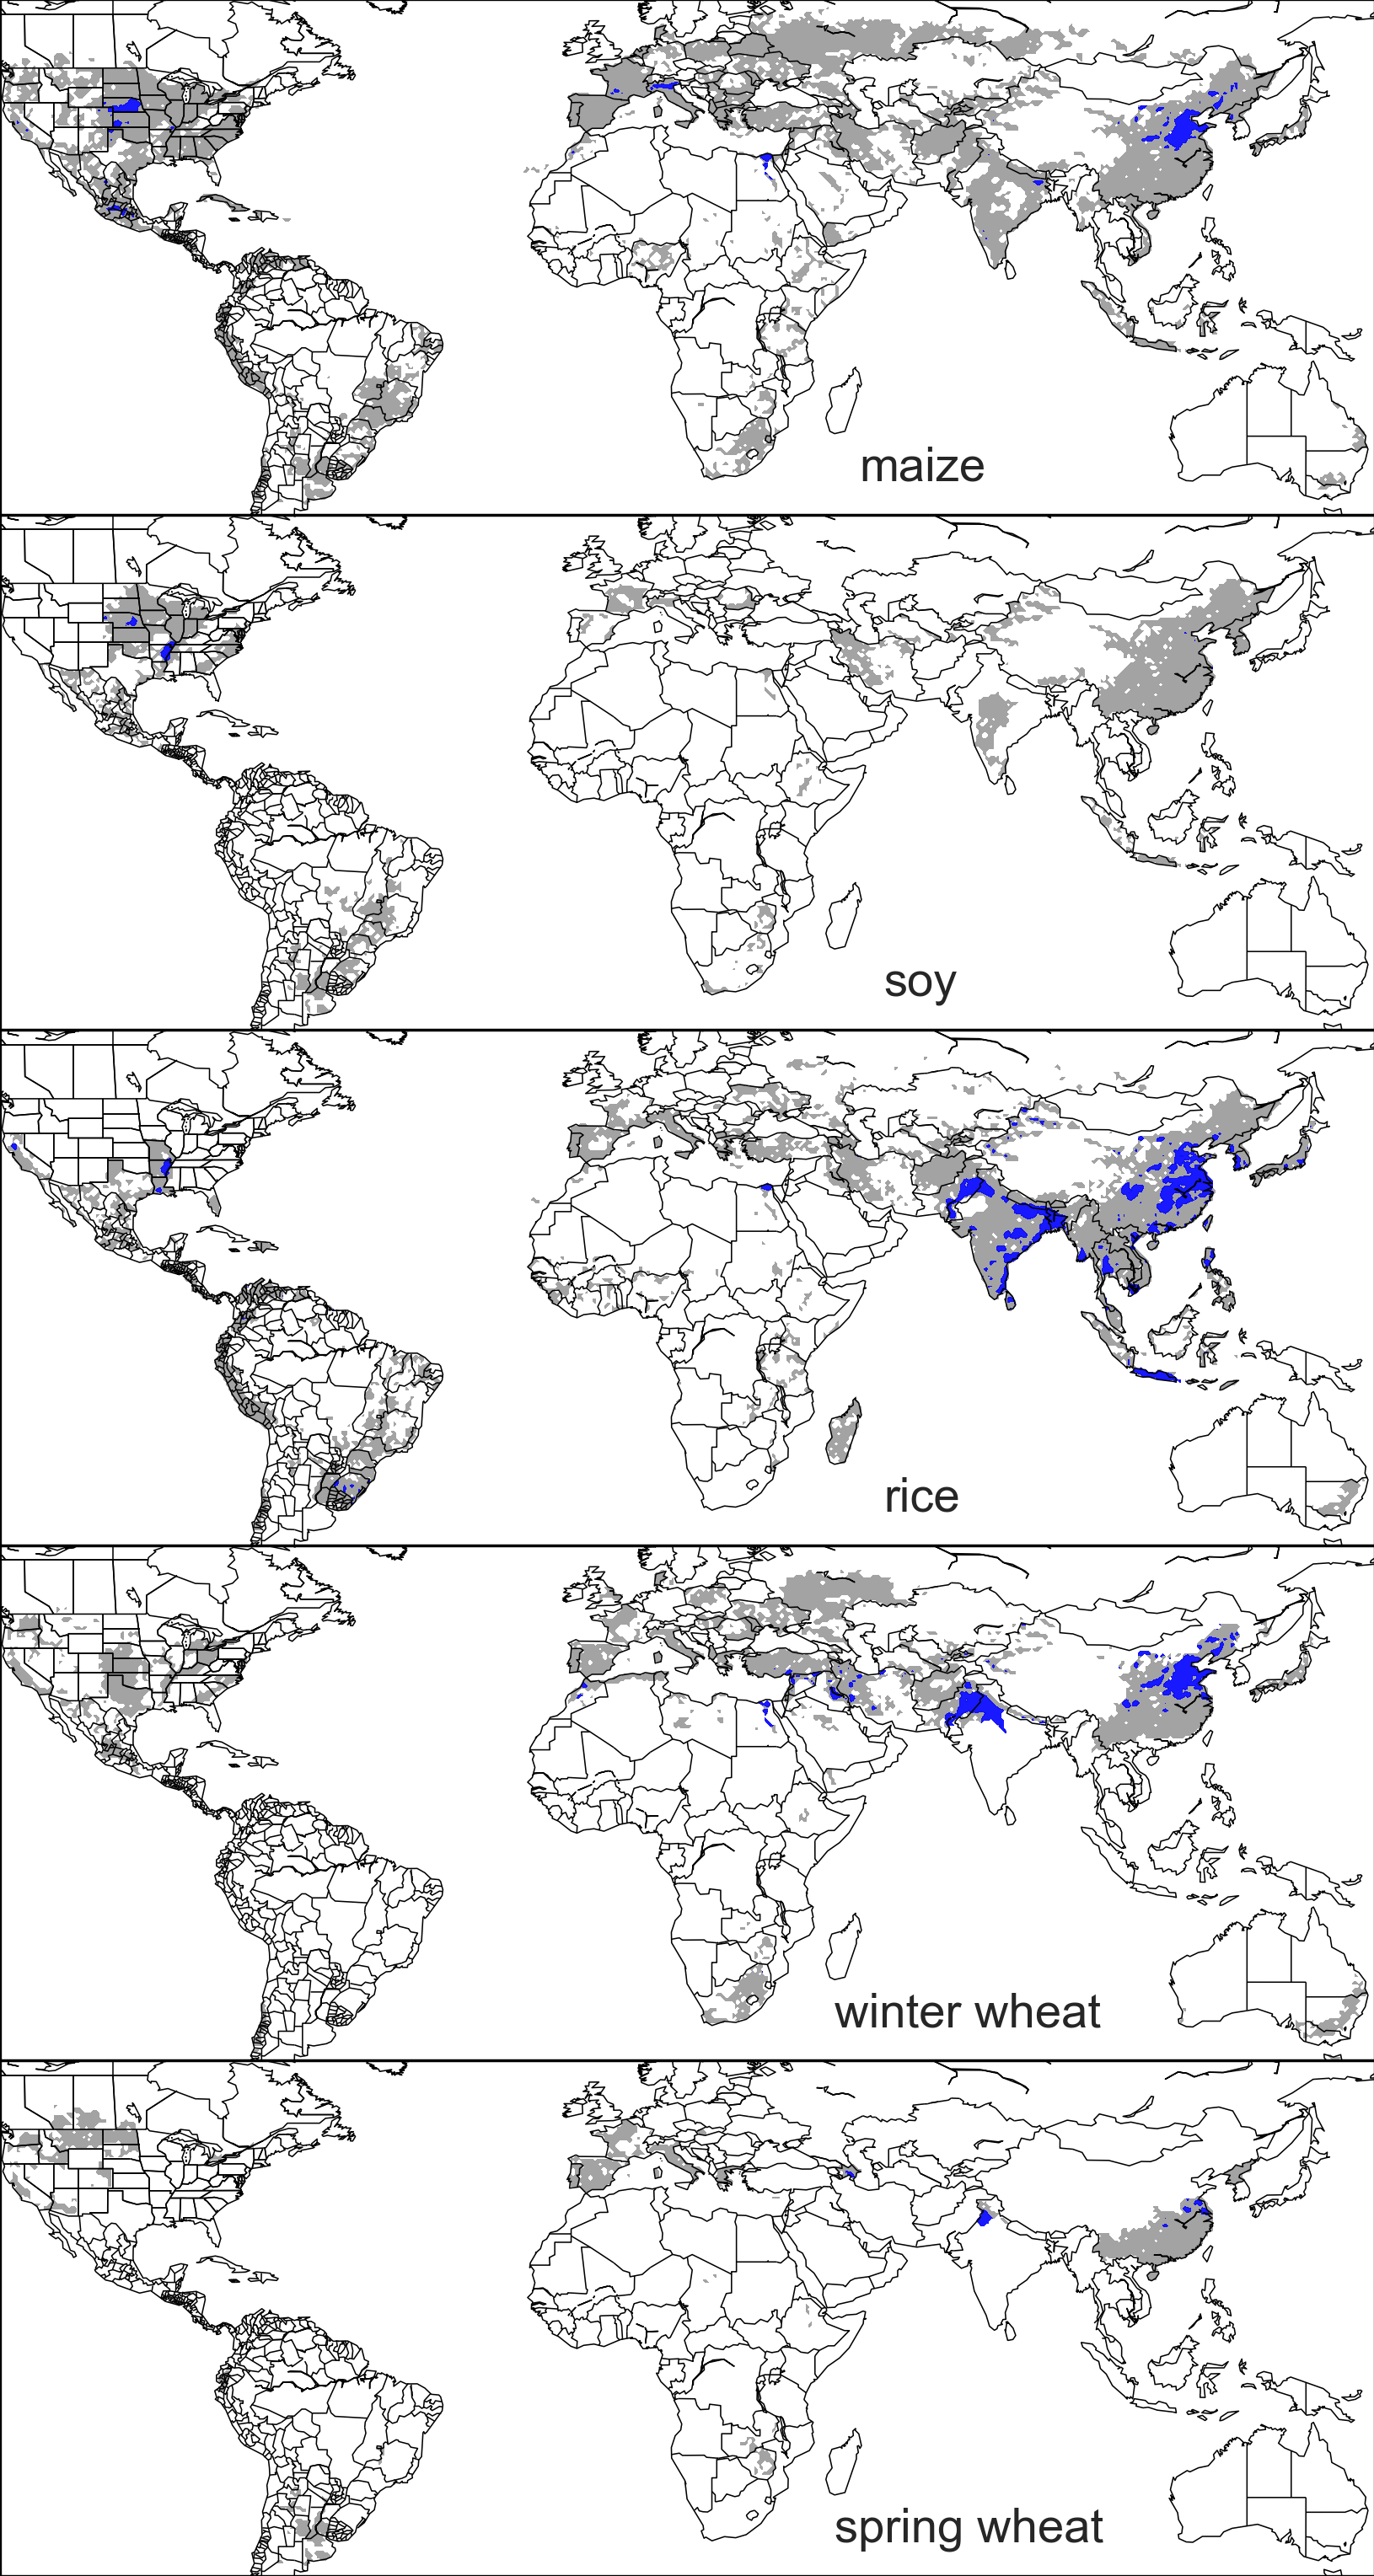
\includegraphics[width=\textwidth]{s_croparea_irr.png}\\
    \caption{Presently cultivated area for irrigated crops in the real world. The blue contour area indicates grid-cells with more that 20,00 hectares of crop cultivated. The gray contour shows area with more that 10 hectares cultivated. Data from the MIRCA2000 data set for maize, rice, and soy. Winter and spring wheat areas are adapted from MIRCA2000 data and sorted by growing season.}
    \label{fig:irrarea}
\end{minipage}
\hspace{.05\linewidth}
%S2
\begin{minipage}{.45\textwidth}
    \centering
    \vspace{-19mm}
    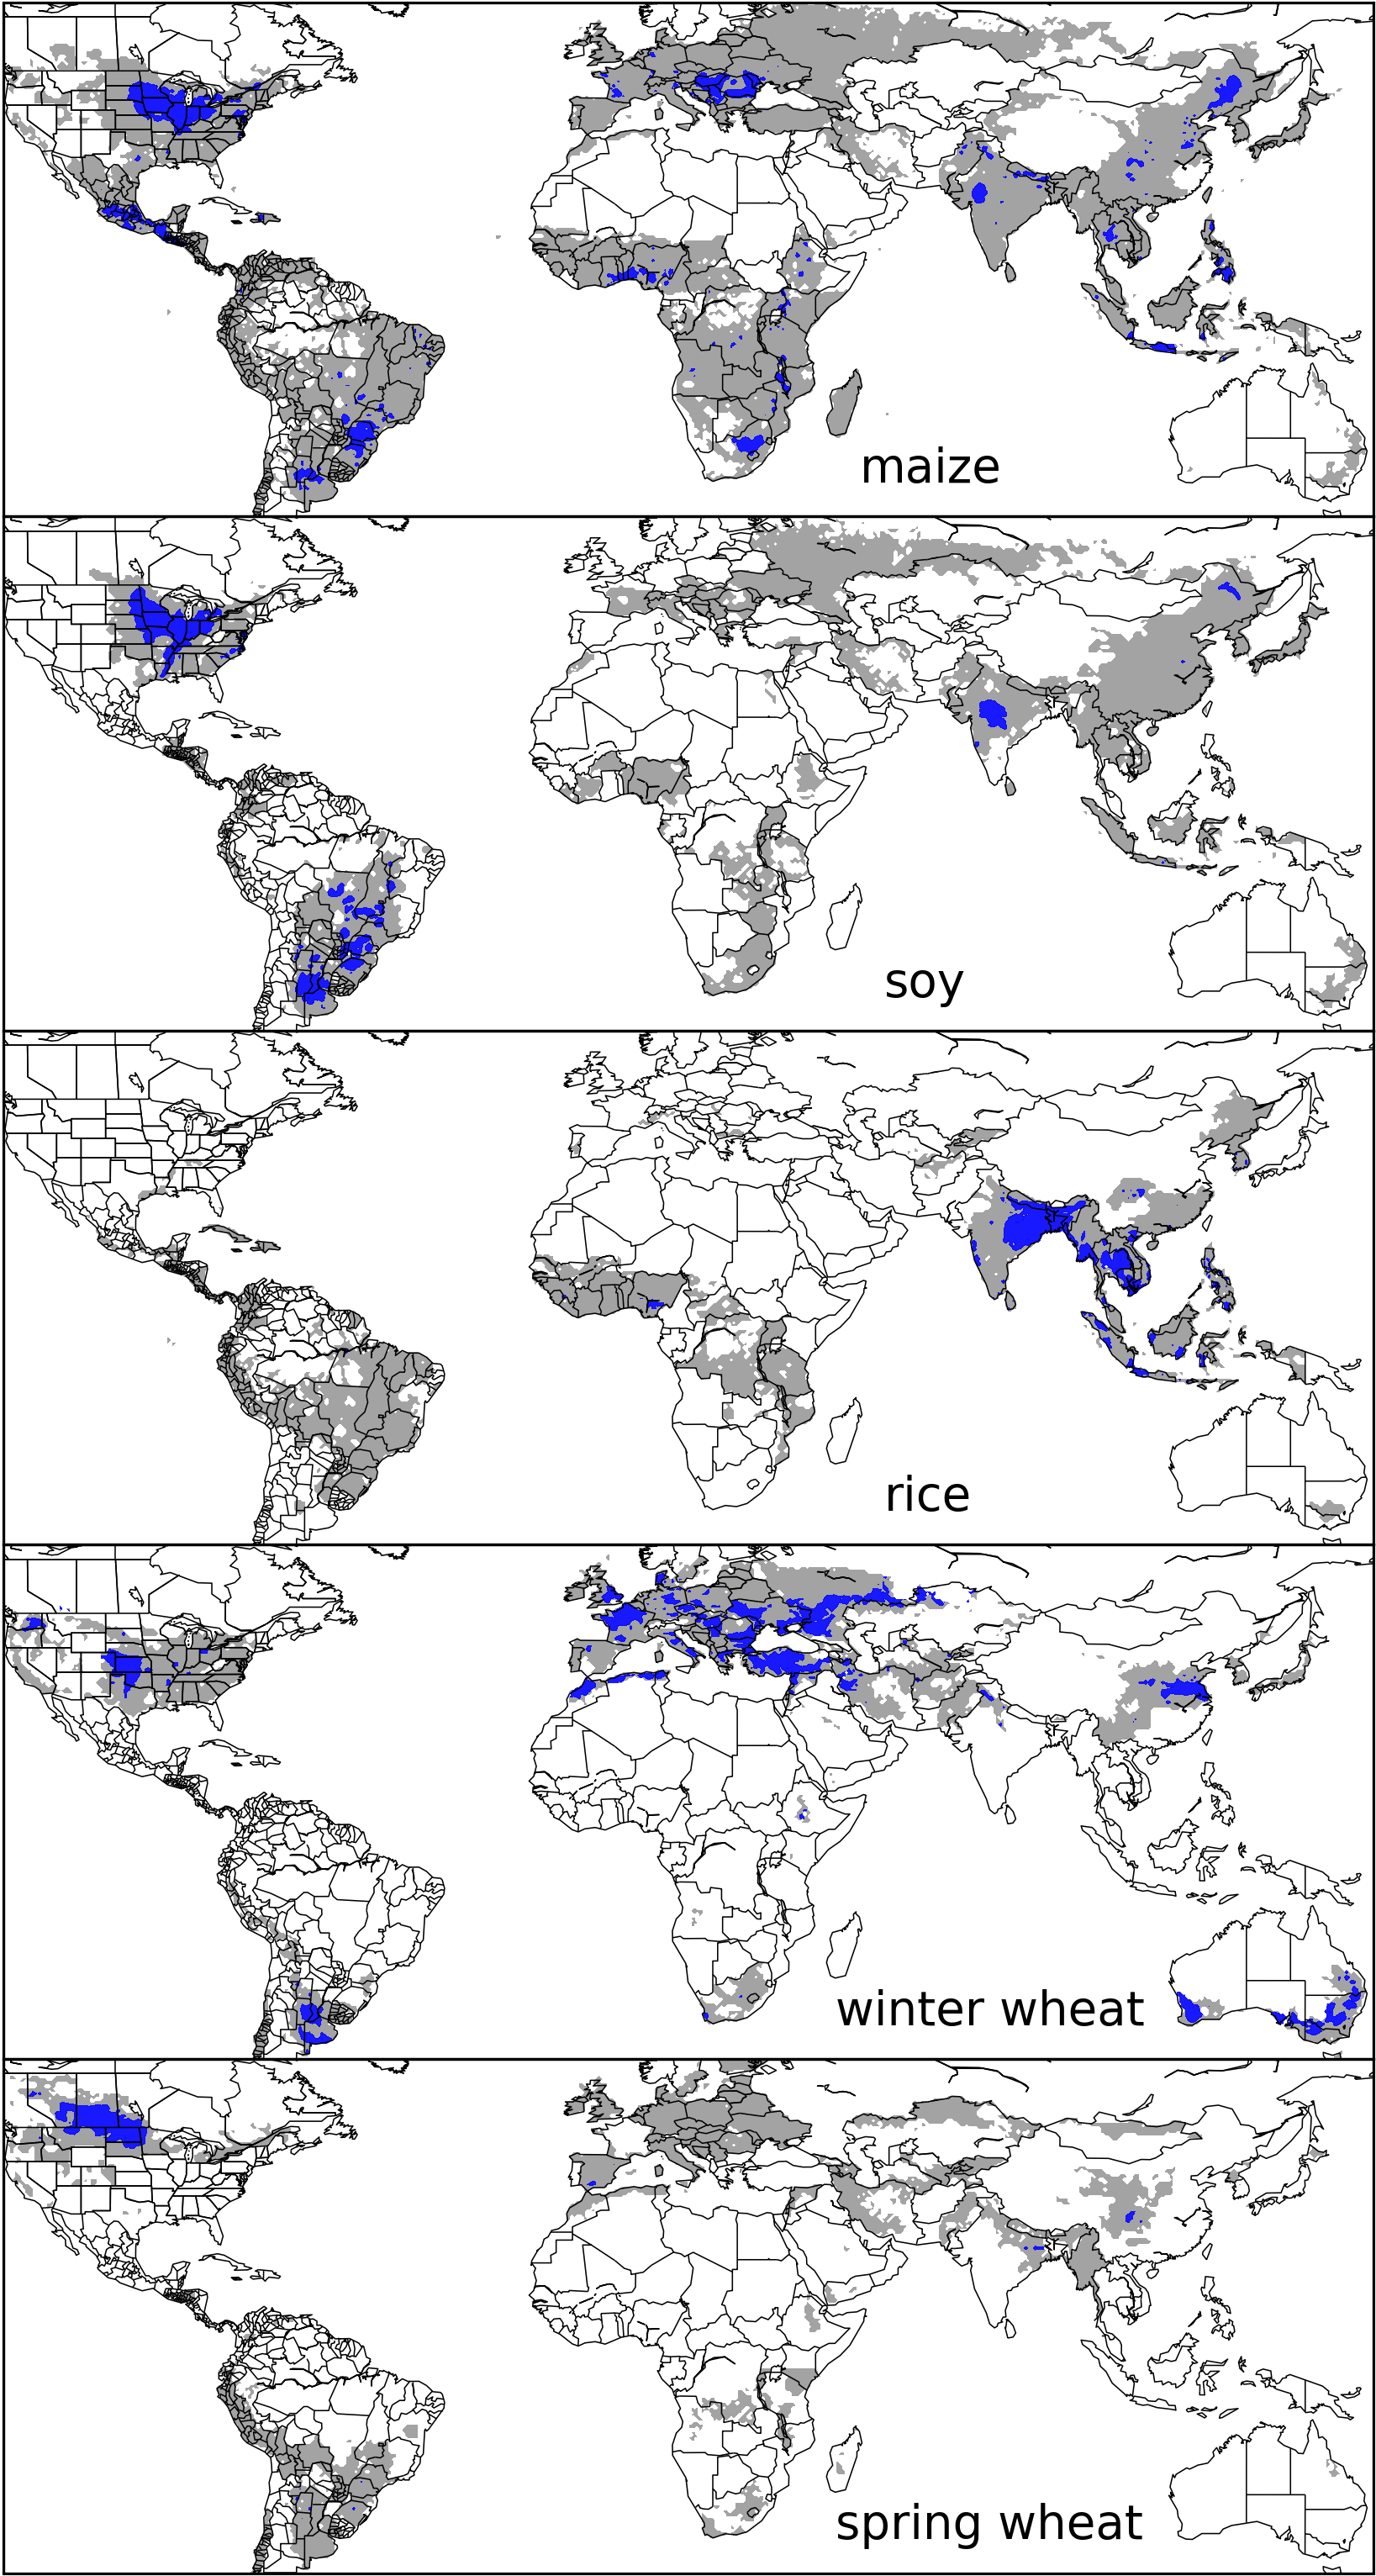
\includegraphics[width=\textwidth]{s_croparea.png}\\
    \caption{Presently cultivated area for rain fed crops in the real world. Conventions as in Figure S1. This figure repeats manuscript Figure 1 for ease of comparison.}
    \label{fig:rainfed}
\end{minipage}
\end{figure}

\section{Experiment Simulation Sampling in Variable Space}
\begin{figure}[h!]
%S3
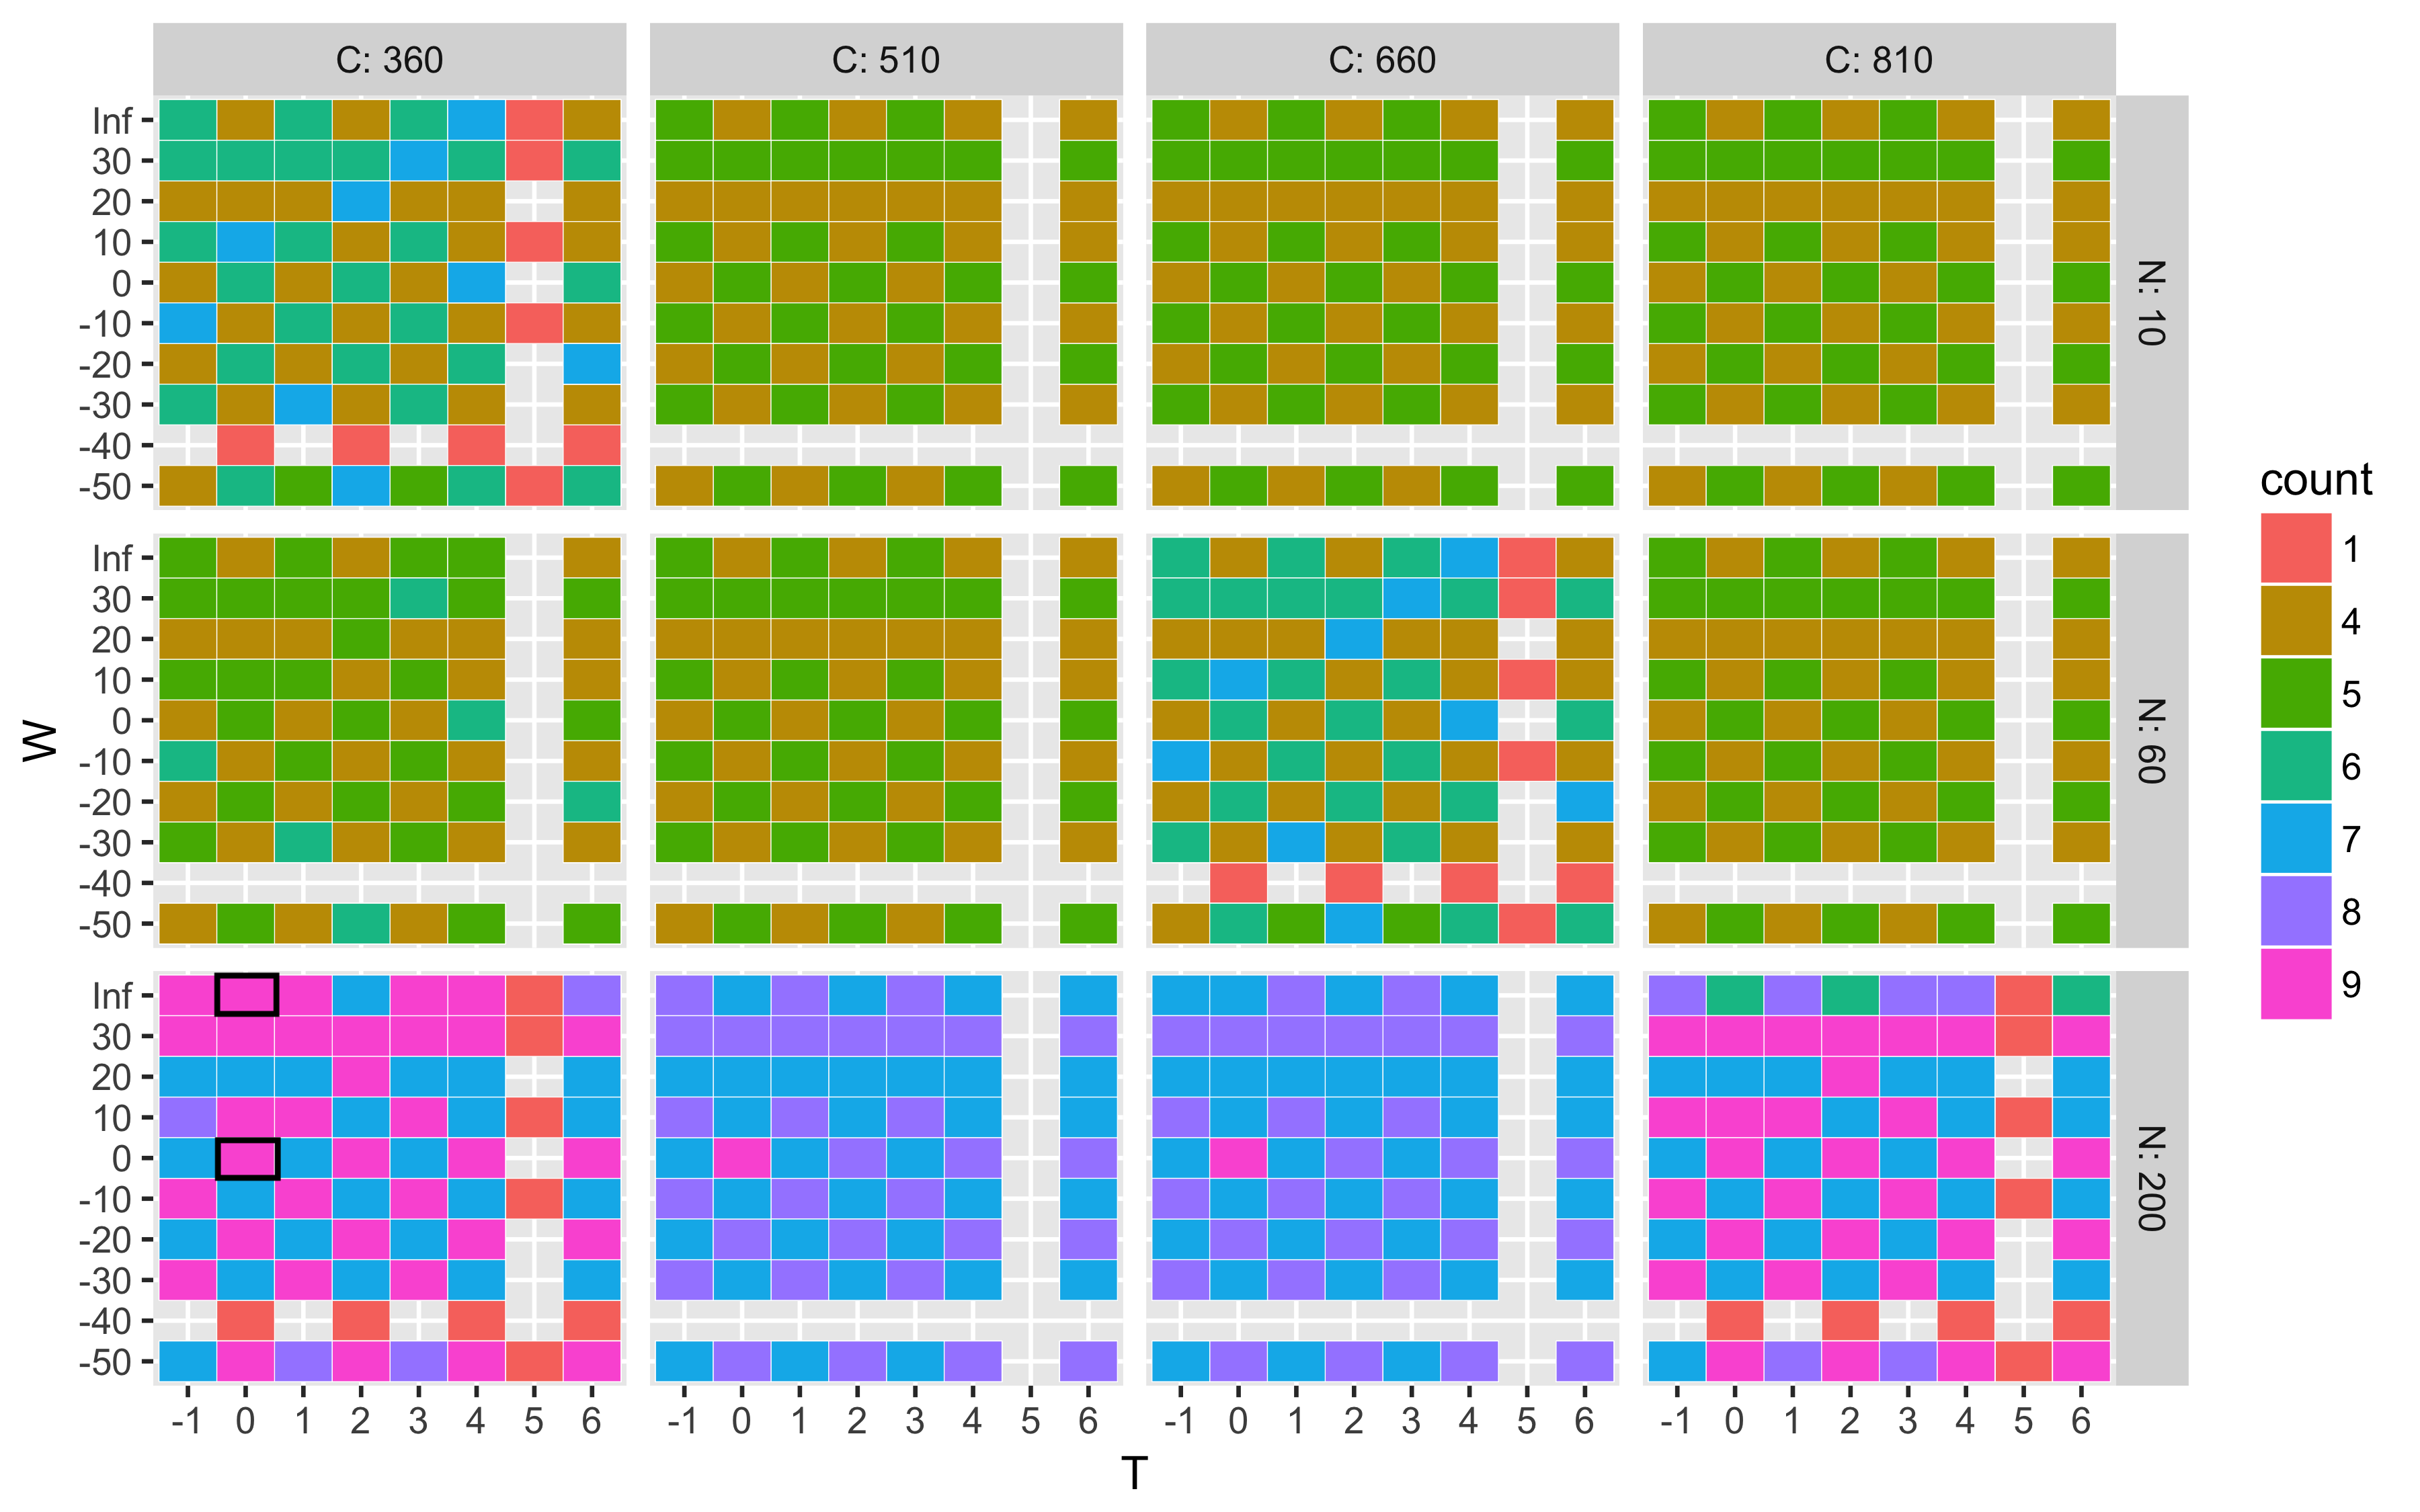
\includegraphics[width=\textwidth]{s_how_many_simulations.png}\\
\caption{Tile heatmap illustrates number of model simulations provided for each of the scenarios in the variable space. The max number is 9, the number of models included in the emulator analysis (excluding three models not included in the emulator analysis). Error calculations are run over scenarios with max number of models (See Figures S25, S26).}
\label{fig:numbersims}
\end{figure}

\clearpage
\section{Maize Simulations}
\begin{figure}[h!]
%S4
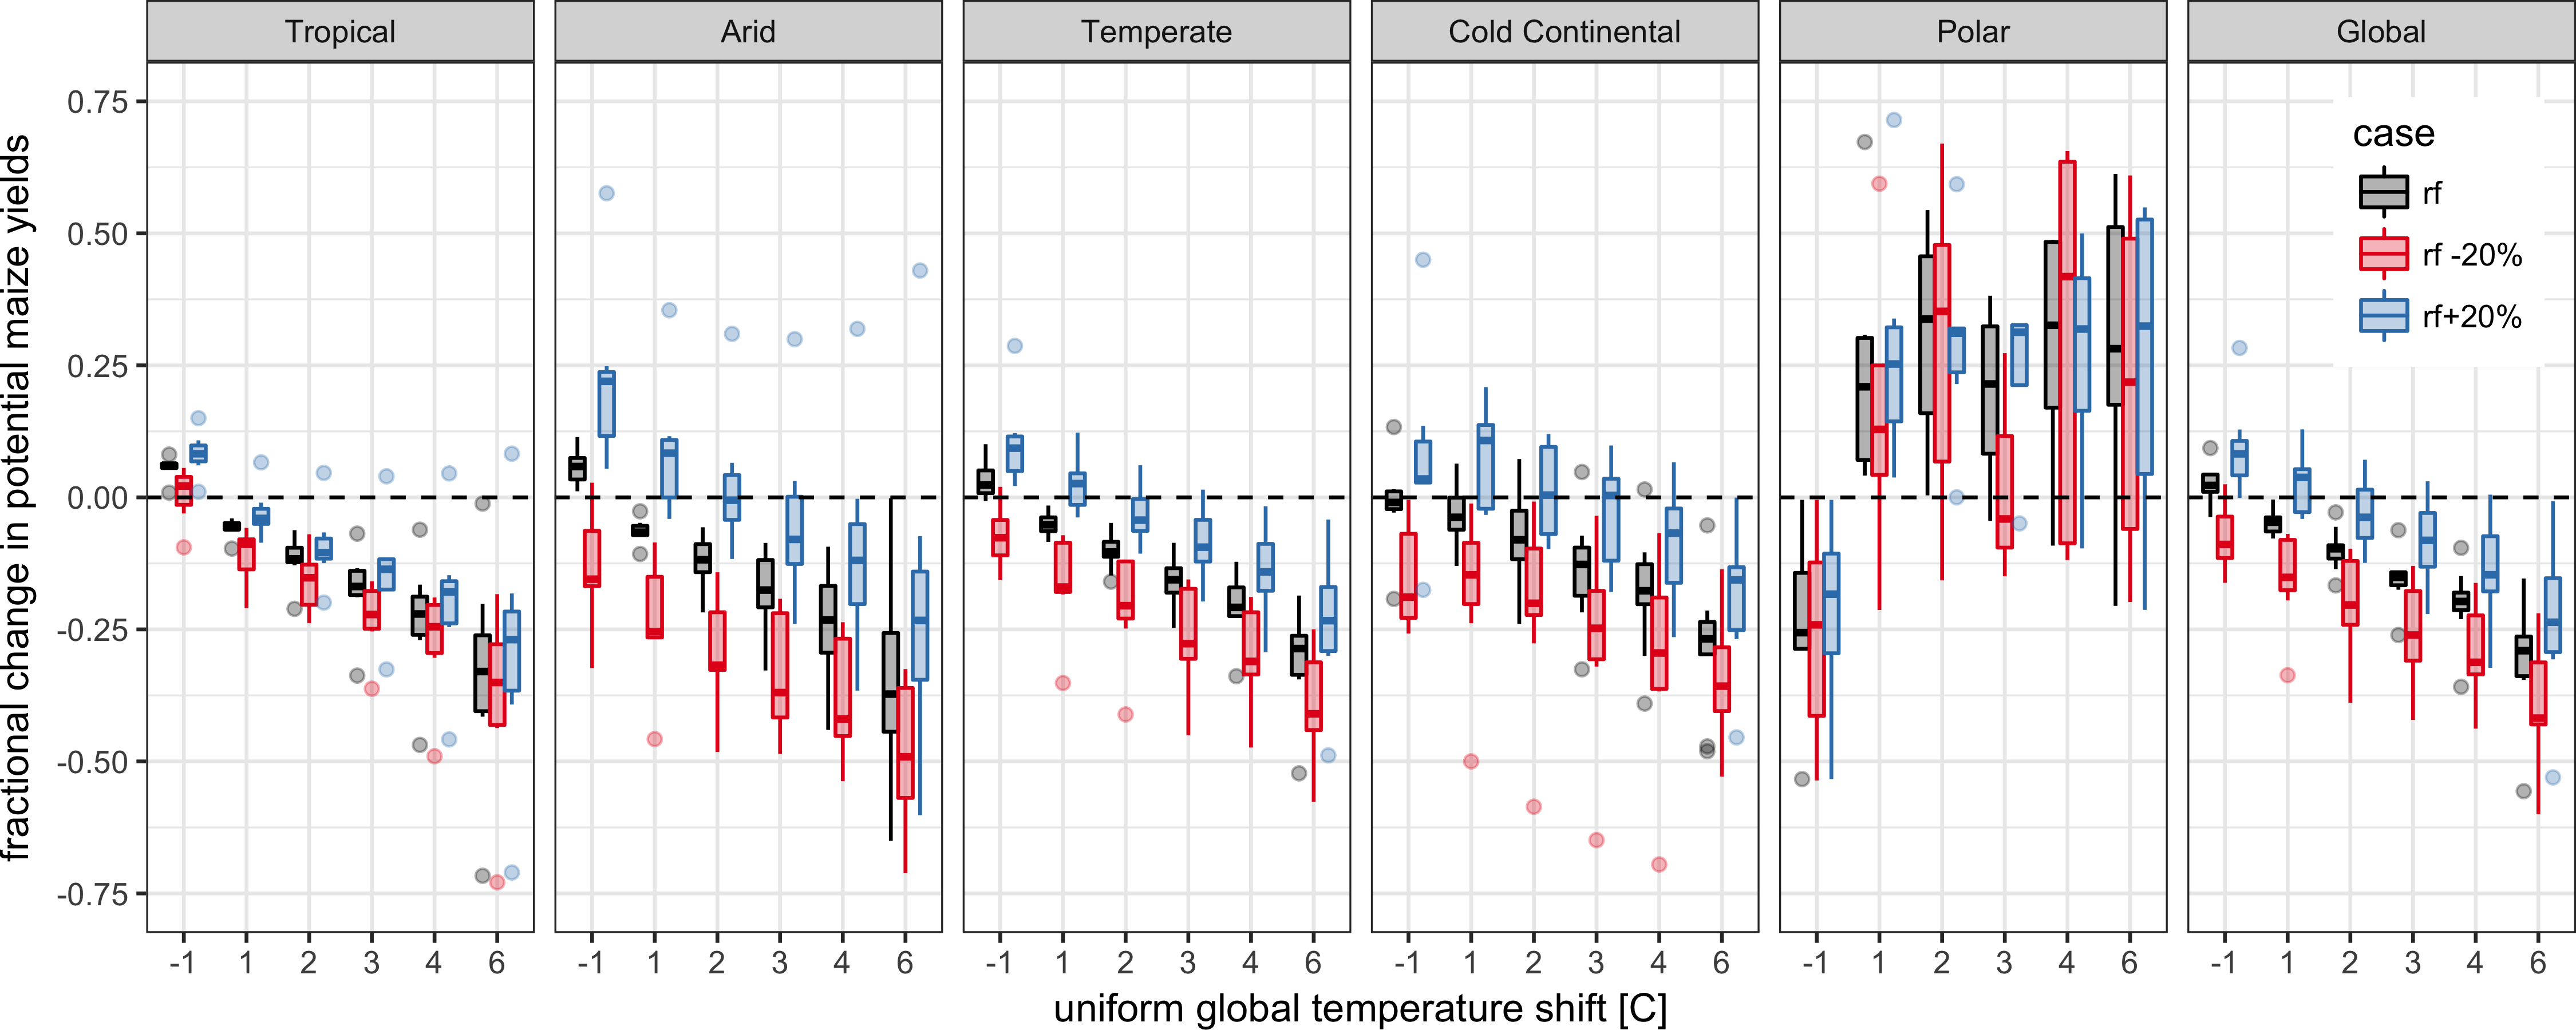
\includegraphics[width=\textwidth]{s_maize_sim_CG_area_weight_rf.png}\\
\caption{Maize simulation results. As in Figure 2 in the main text but weighted by actual cultivation area in the real world instead of across all grid cells. Additional figure conventions are the same as Figure 2 in the main text. All other covariates are held constant.}
\label{fig:KGirr_currentcult}
\end{figure}
\section{All Crops Simulations}
\begin{figure}[h!]
%S5
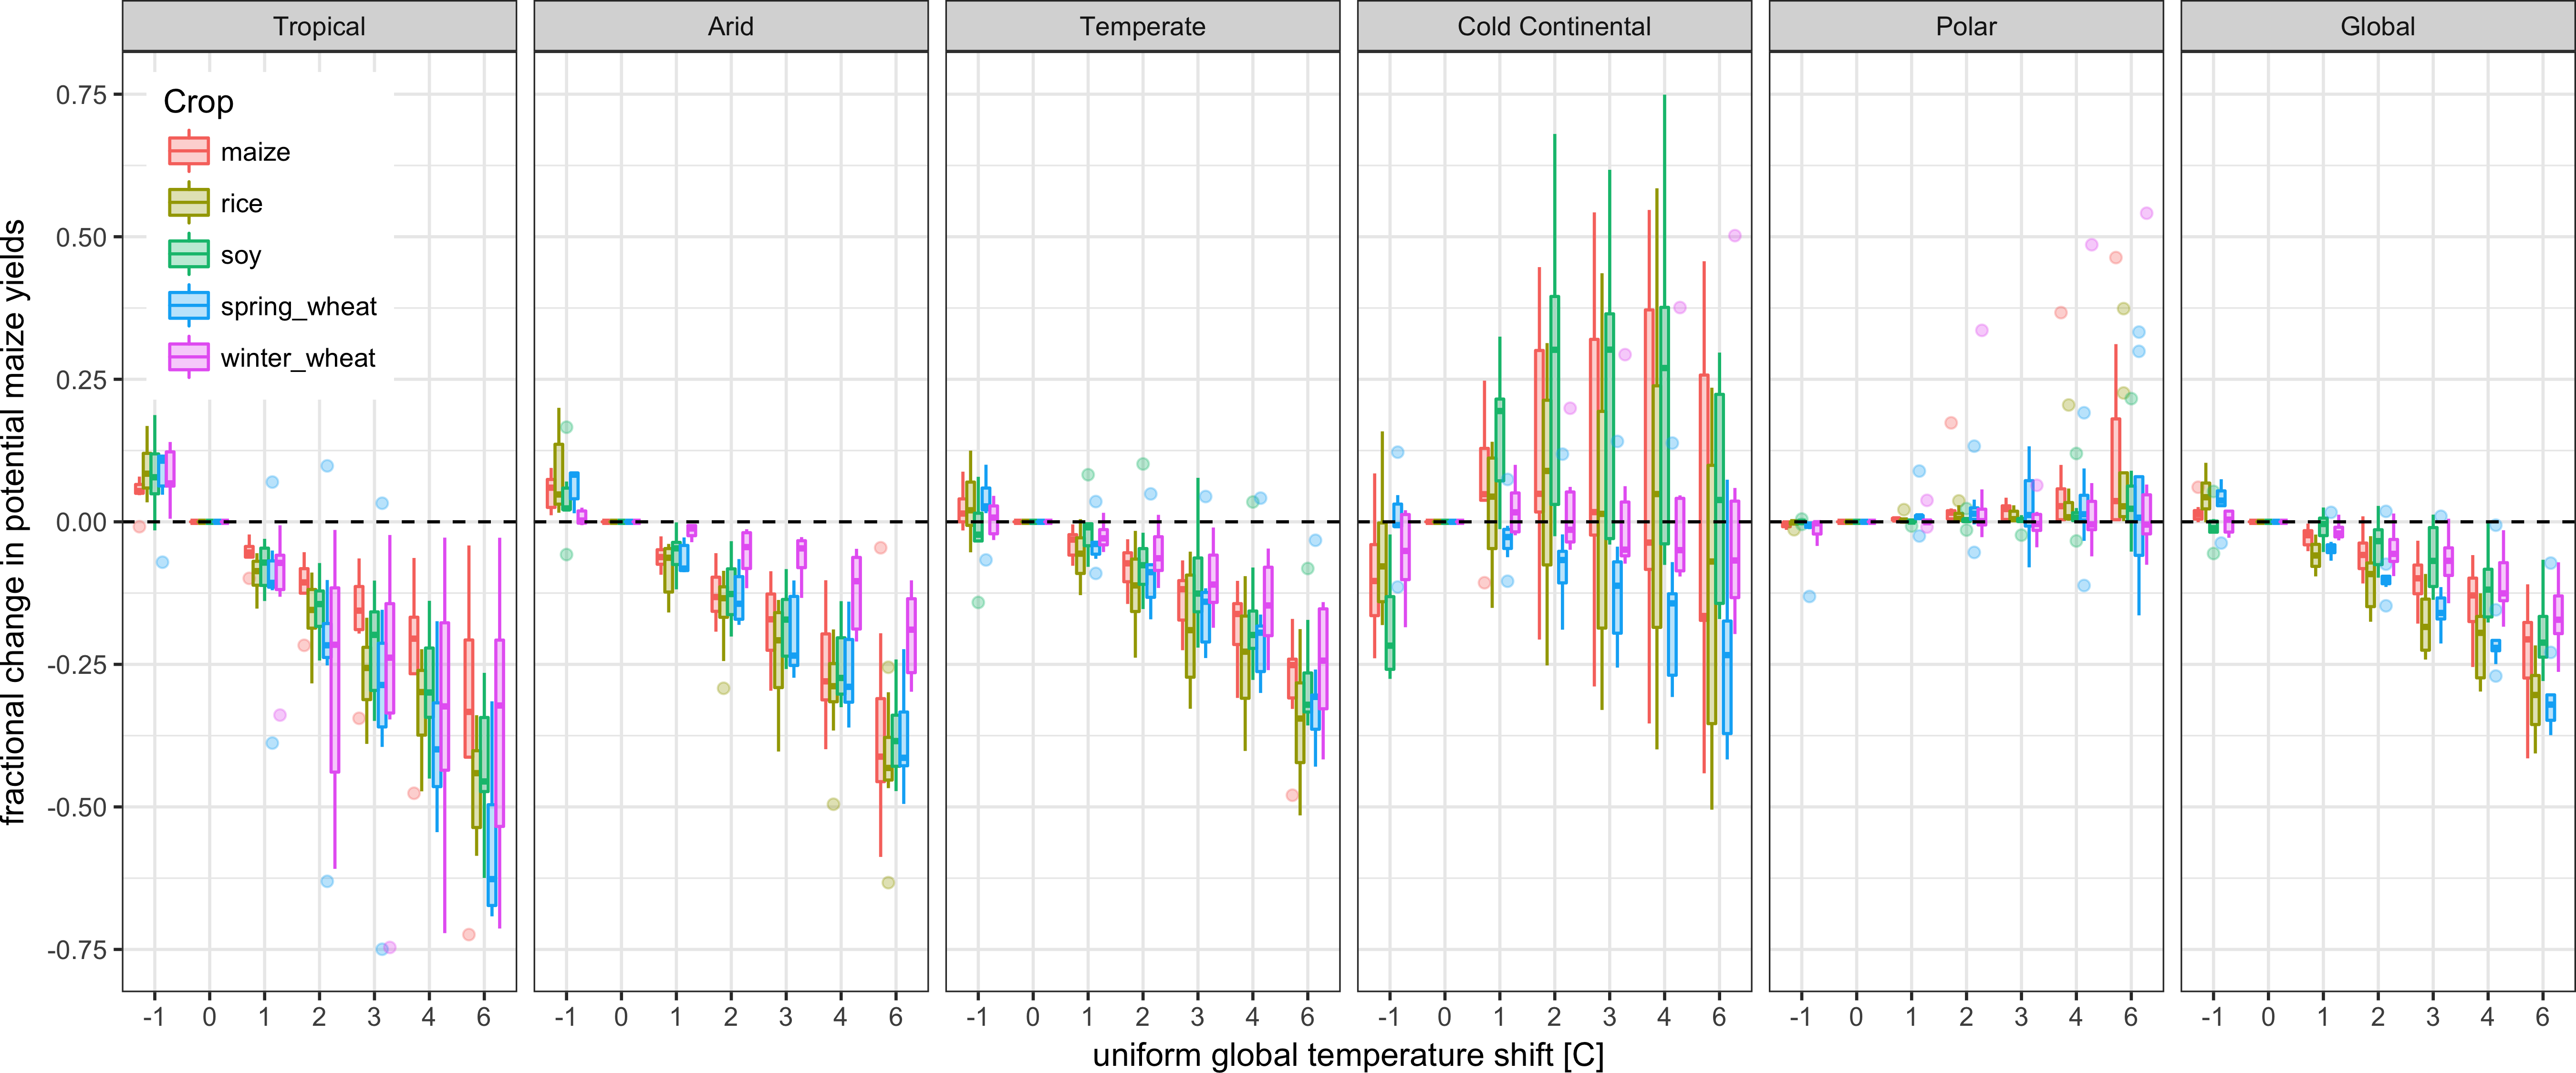
\includegraphics[width=\textwidth]{s_sim_KG_crops_all.png}\\
\caption{All crop simulation results. As in Figure 2 in the main document except for all models for the rainfed case (without -20 or +20\% rainfall as in Figure 2 in main text.) In cold continental regions, soy yields generally increase with warming and spring wheat yields decrease; the other crops are indeterminate across models. All other covariates are held constant.}
\label{fig:KGcrops_all}
\end{figure}

\clearpage
\section{Maize Simulations}
\subsection{All grid cells}
\begin{figure}[h!]
%S7
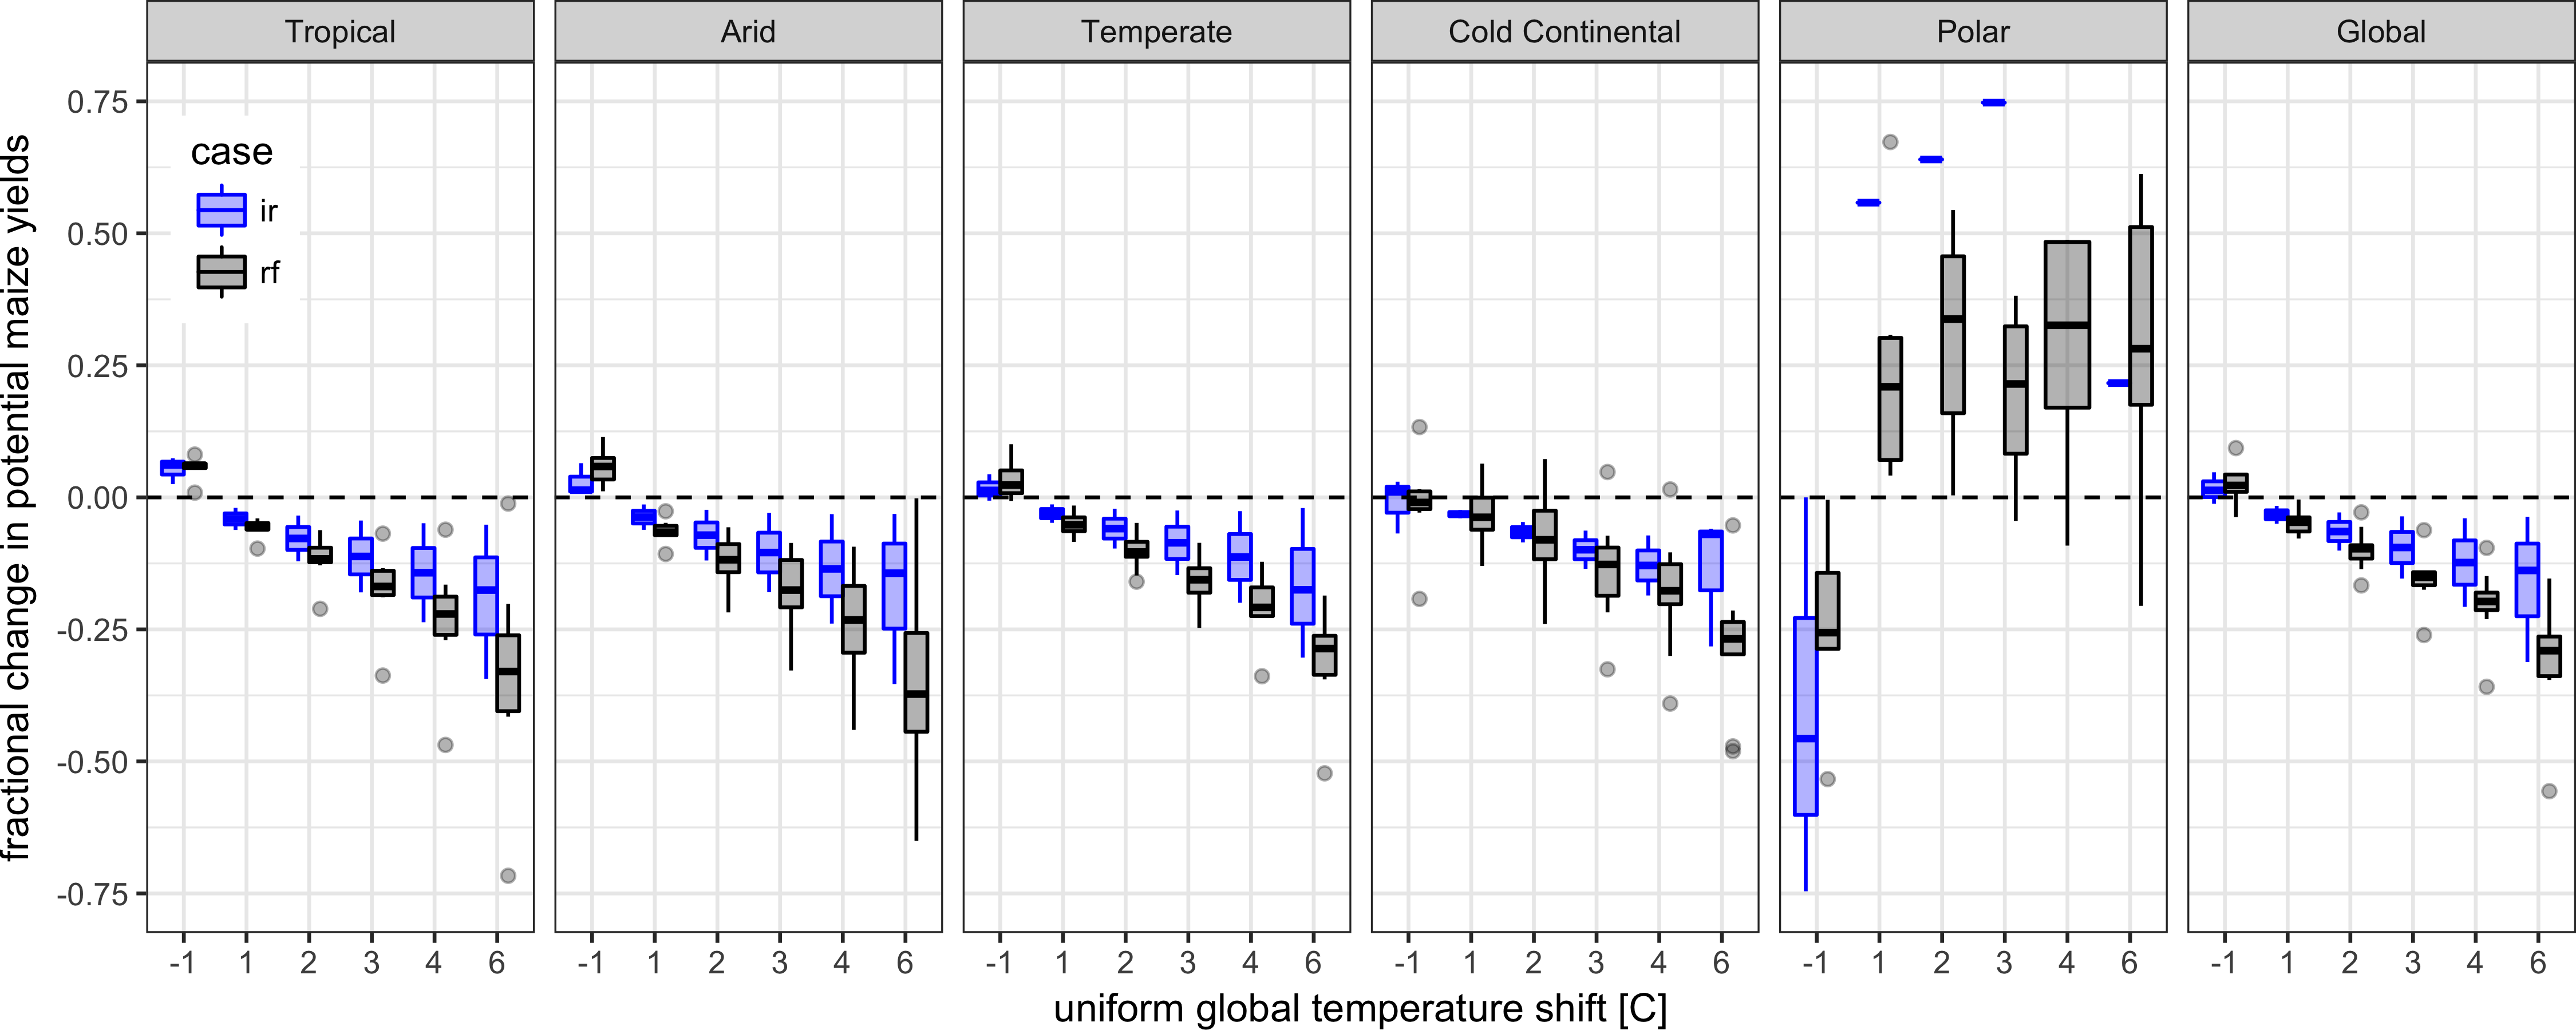
\includegraphics[width=\textwidth]{s_maize_sim_CG.png}\\
\caption{Maize simulation results. As in Figure 2 in the main text except comparing rainfed to irrigated maize across all grid cells. All other figure conventions match Figure 2 in the main text.}
\label{fig:maizeCG}
\end{figure}

\subsection{Currently cultivated area}
\begin{figure}[h!]
%S8
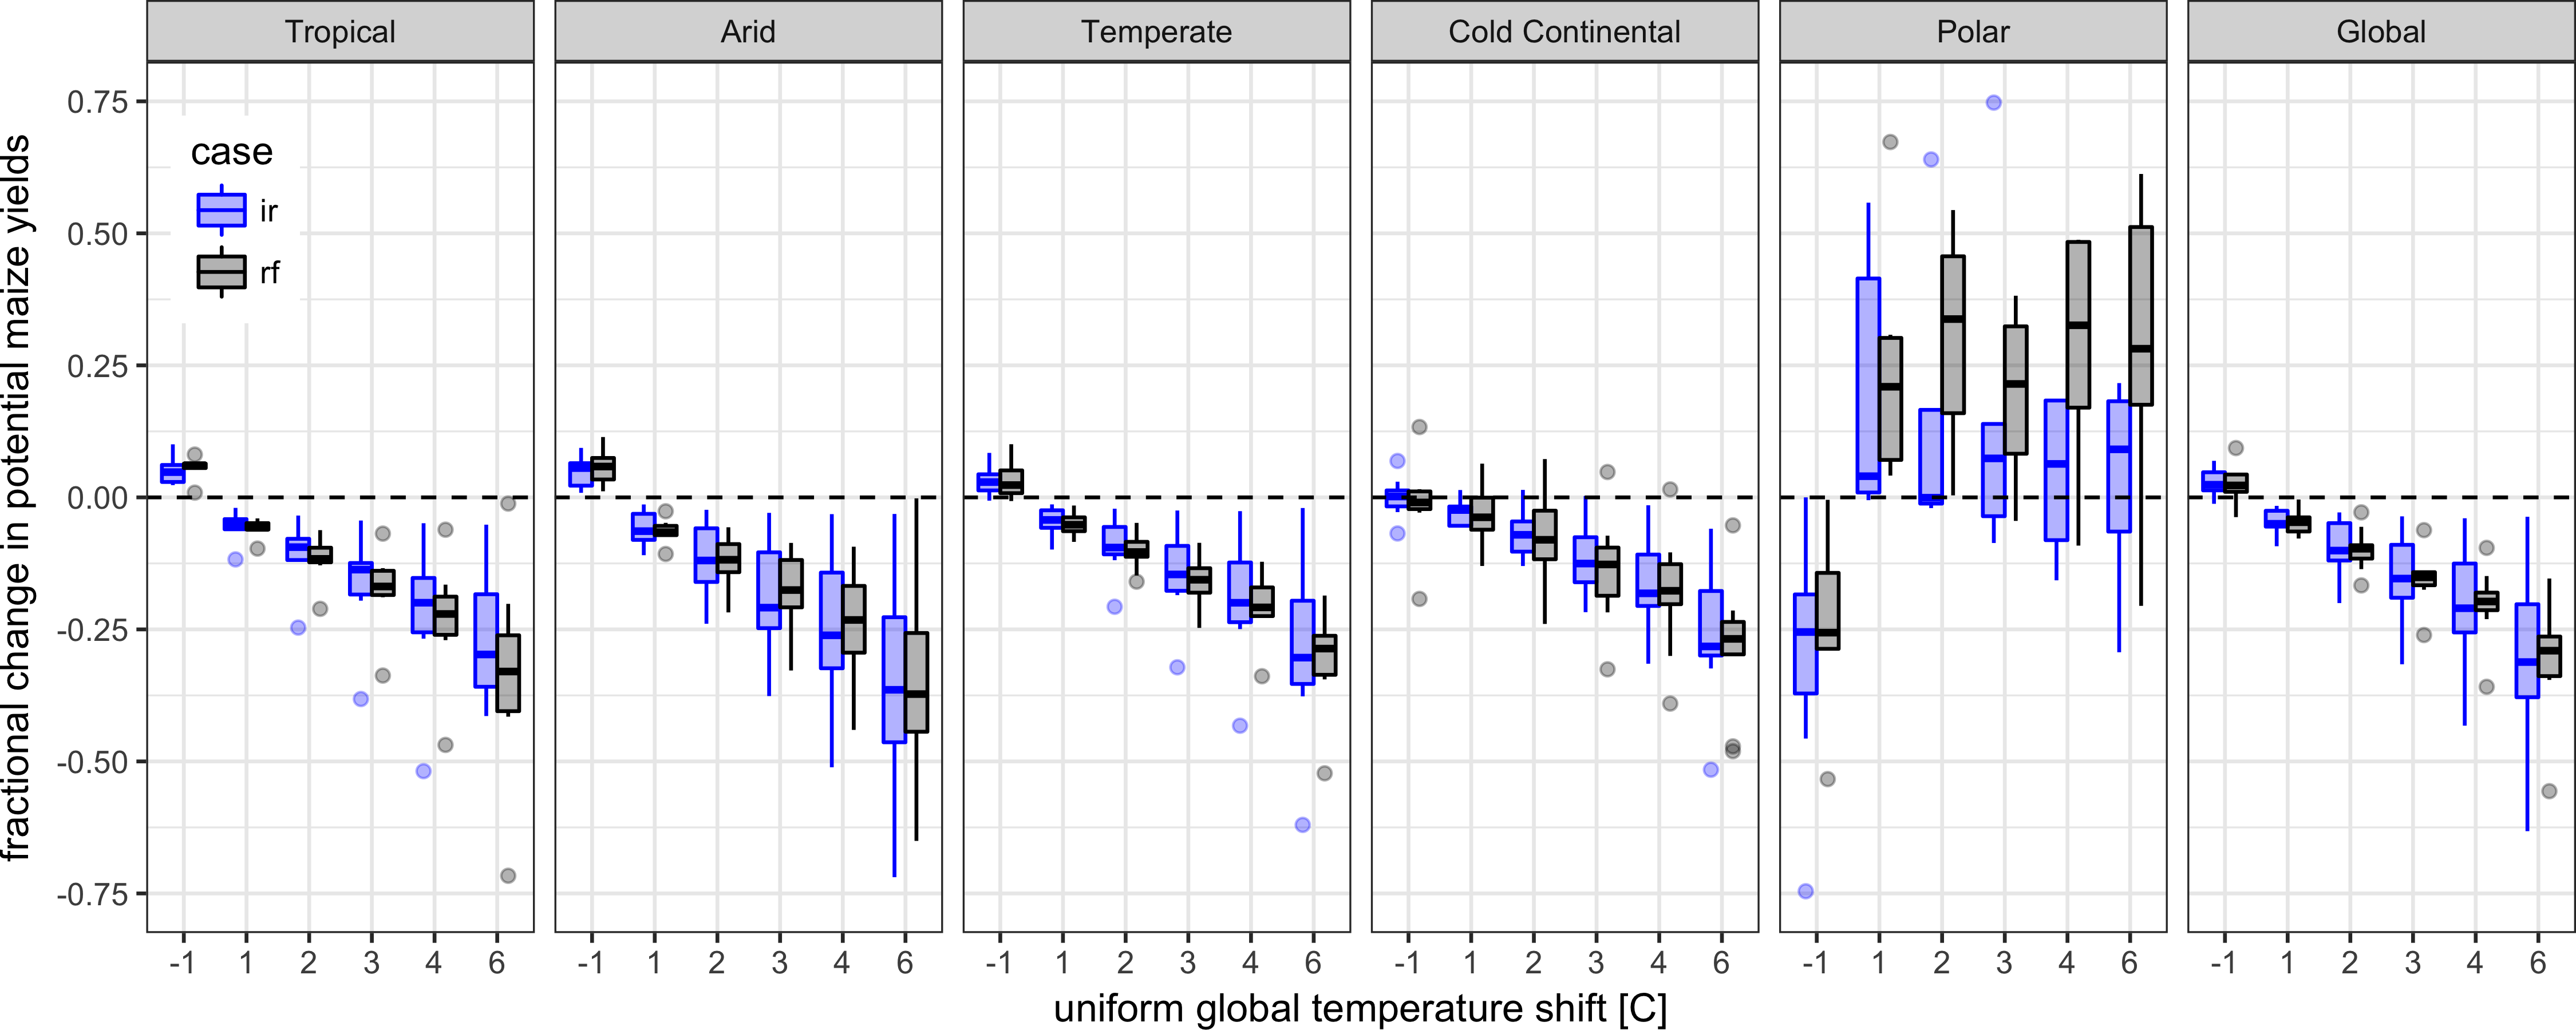
\includegraphics[width=\textwidth]{s_maize_sim_CG_area_weight.png}\\
\caption{Maize simulation results. As in Figure 2 in the main text except comparing rainfed to irrigated maize across currently cultivated hectares. All other figure conventions match Figure 2 in the main text.}
\label{fig:maizeCG}
\end{figure}

\clearpage
\section{Soy Simulations}
\subsection{All grid cells}
\begin{figure}[h!]
%S9
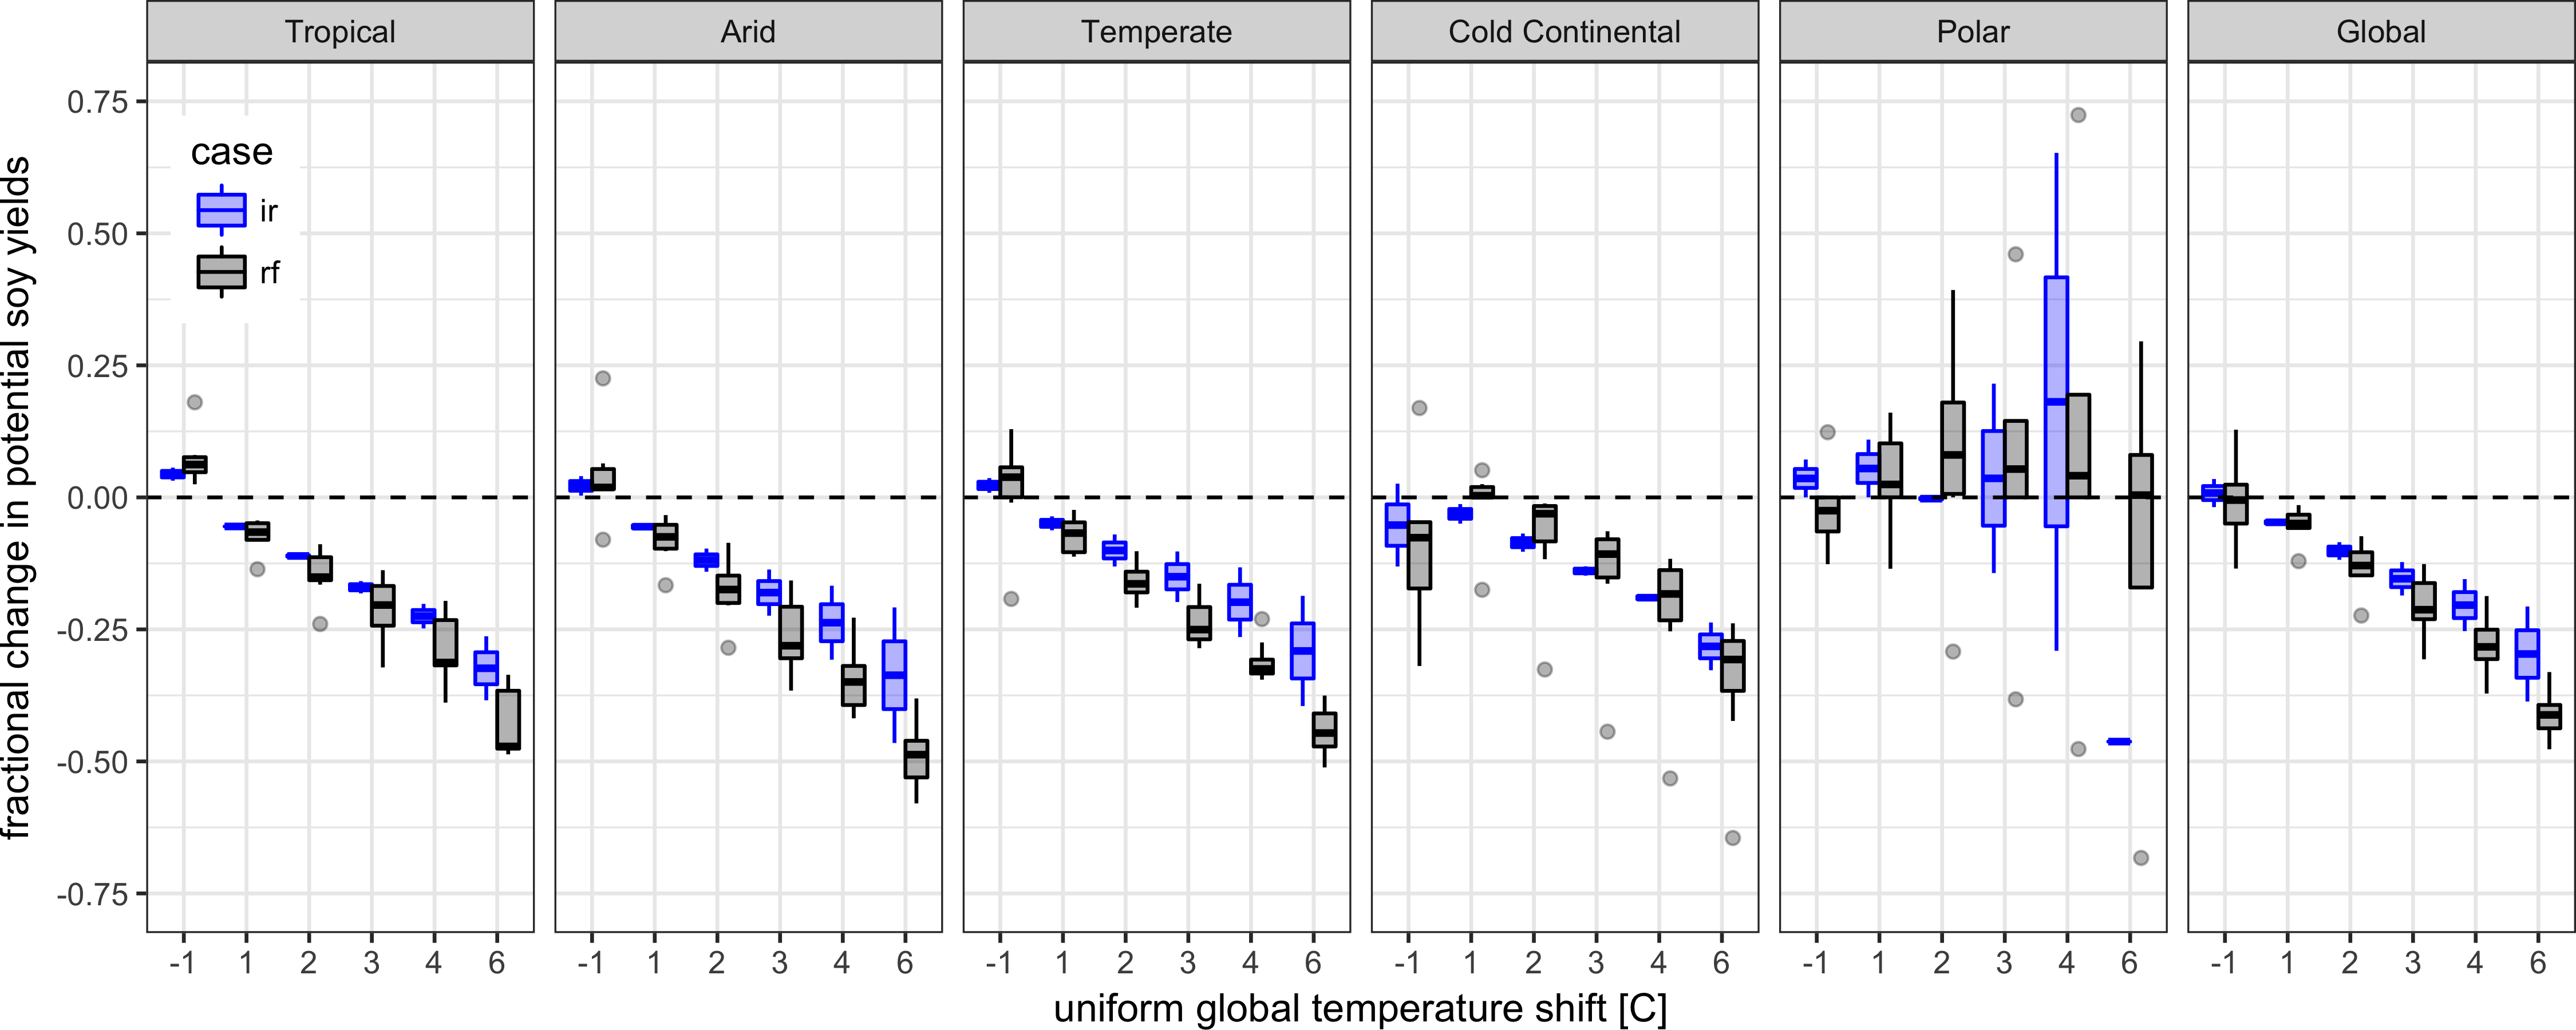
\includegraphics[width=\textwidth]{s_soy_sim_CG.png}\\
\caption{Soy simulation results. As in Figure 2 in the main text except comparing rainfed to irrigated soy across all grid cells. All other figure conventions match Figure 2 in the main text.}
\label{fig:maizeCG}
\end{figure}

\subsection{Currently cultivated area}
\begin{figure}[h!]
%S10
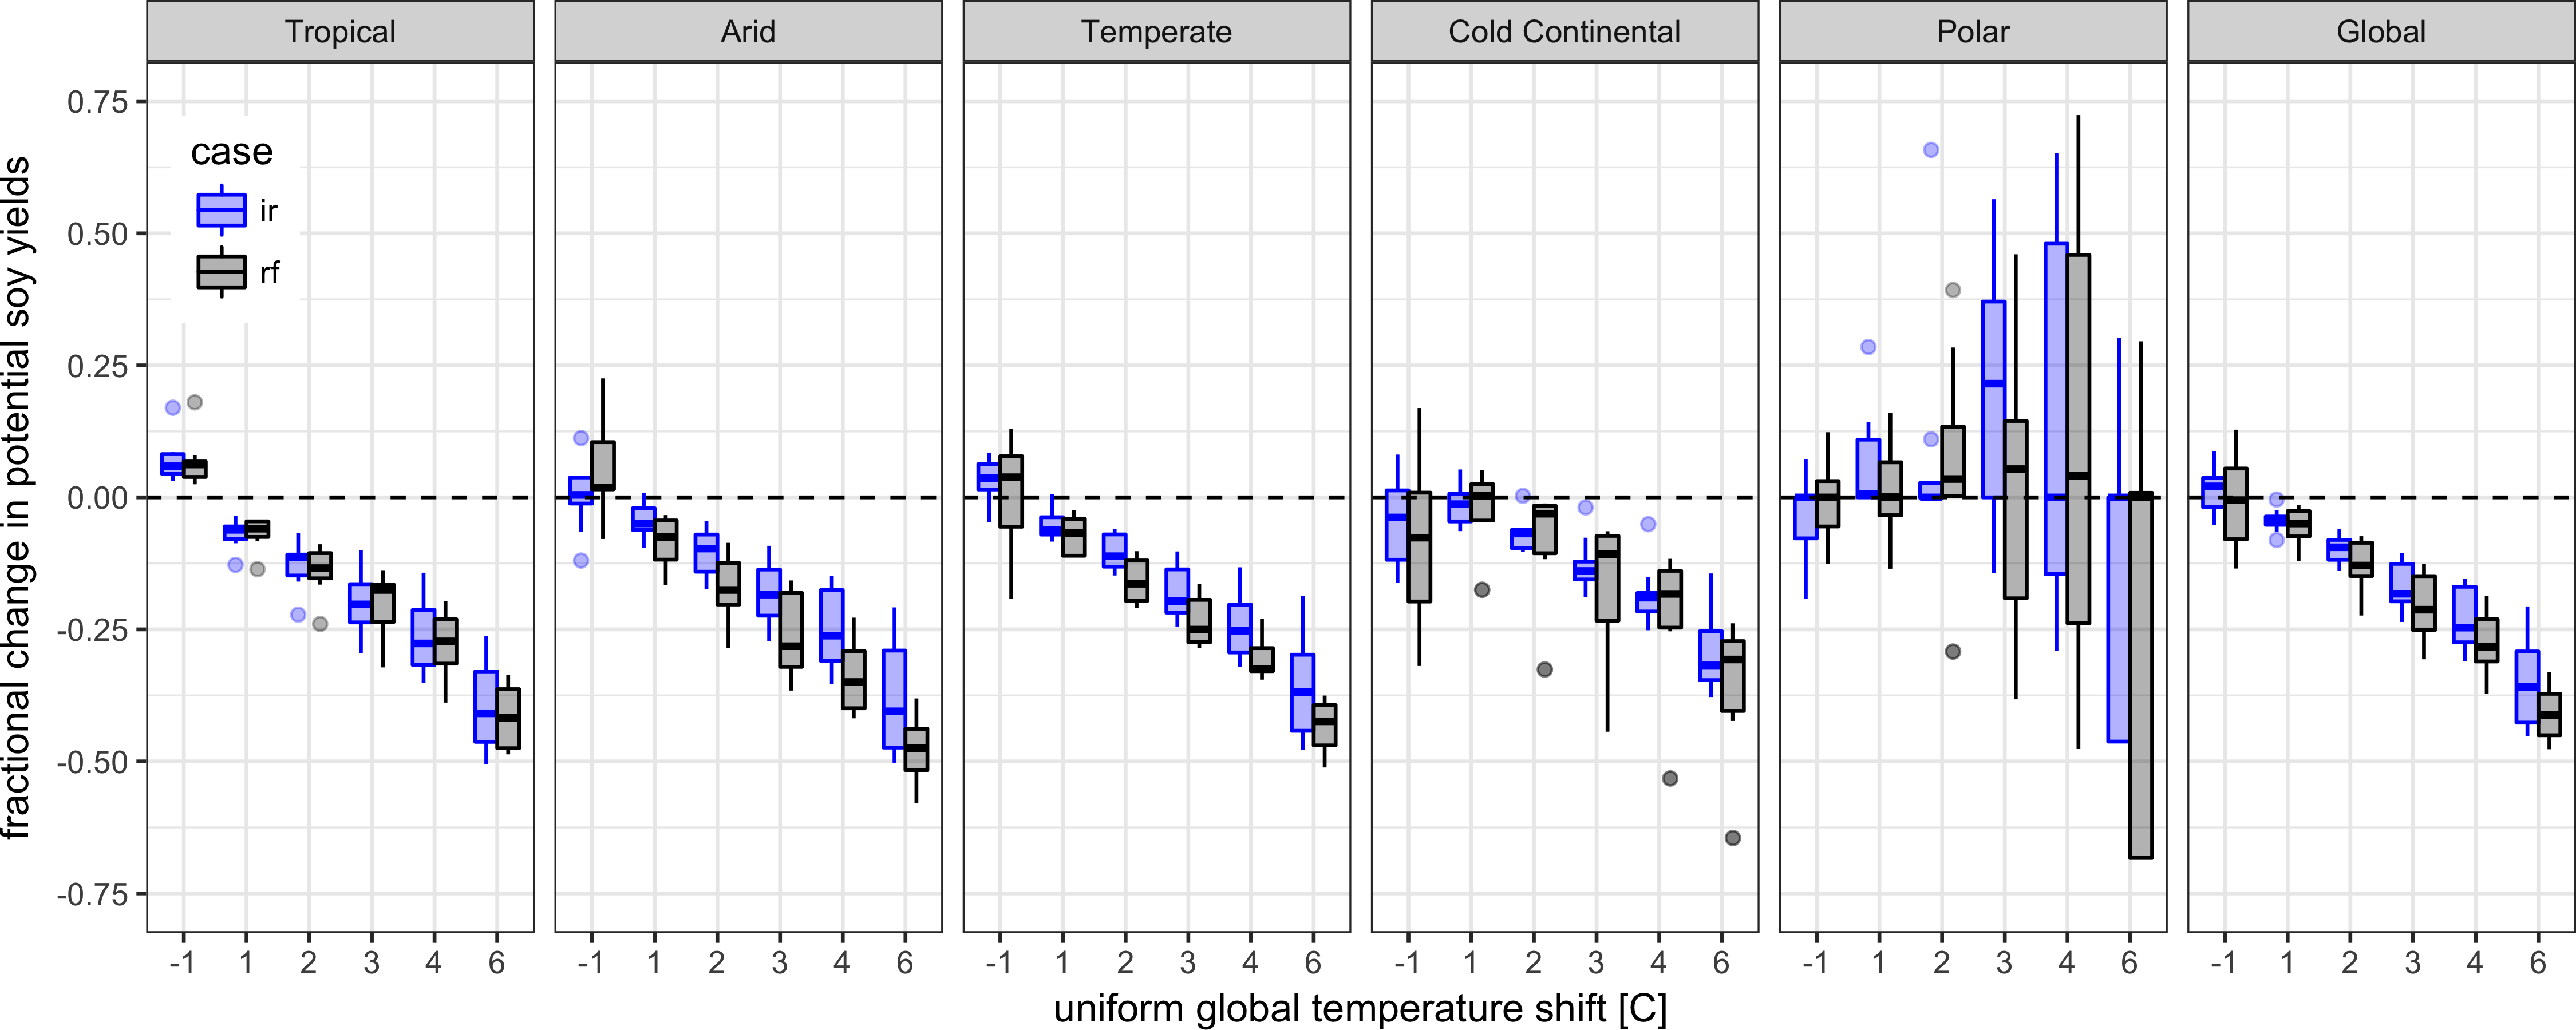
\includegraphics[width=\textwidth]{s_soy_sim_CG_area_weight.png}\\
\caption{Soy simulation results. As in Figure 2 in the main text except comparing rainfed to irrigated soy across currently cultivated hectares. All other figure conventions match Figure 2 in the main text.}
\label{fig:maizeCG}
\end{figure}

\clearpage
\section{Rice Simulations}
\subsection{All grid cells}
\begin{figure}[h!]
%S11
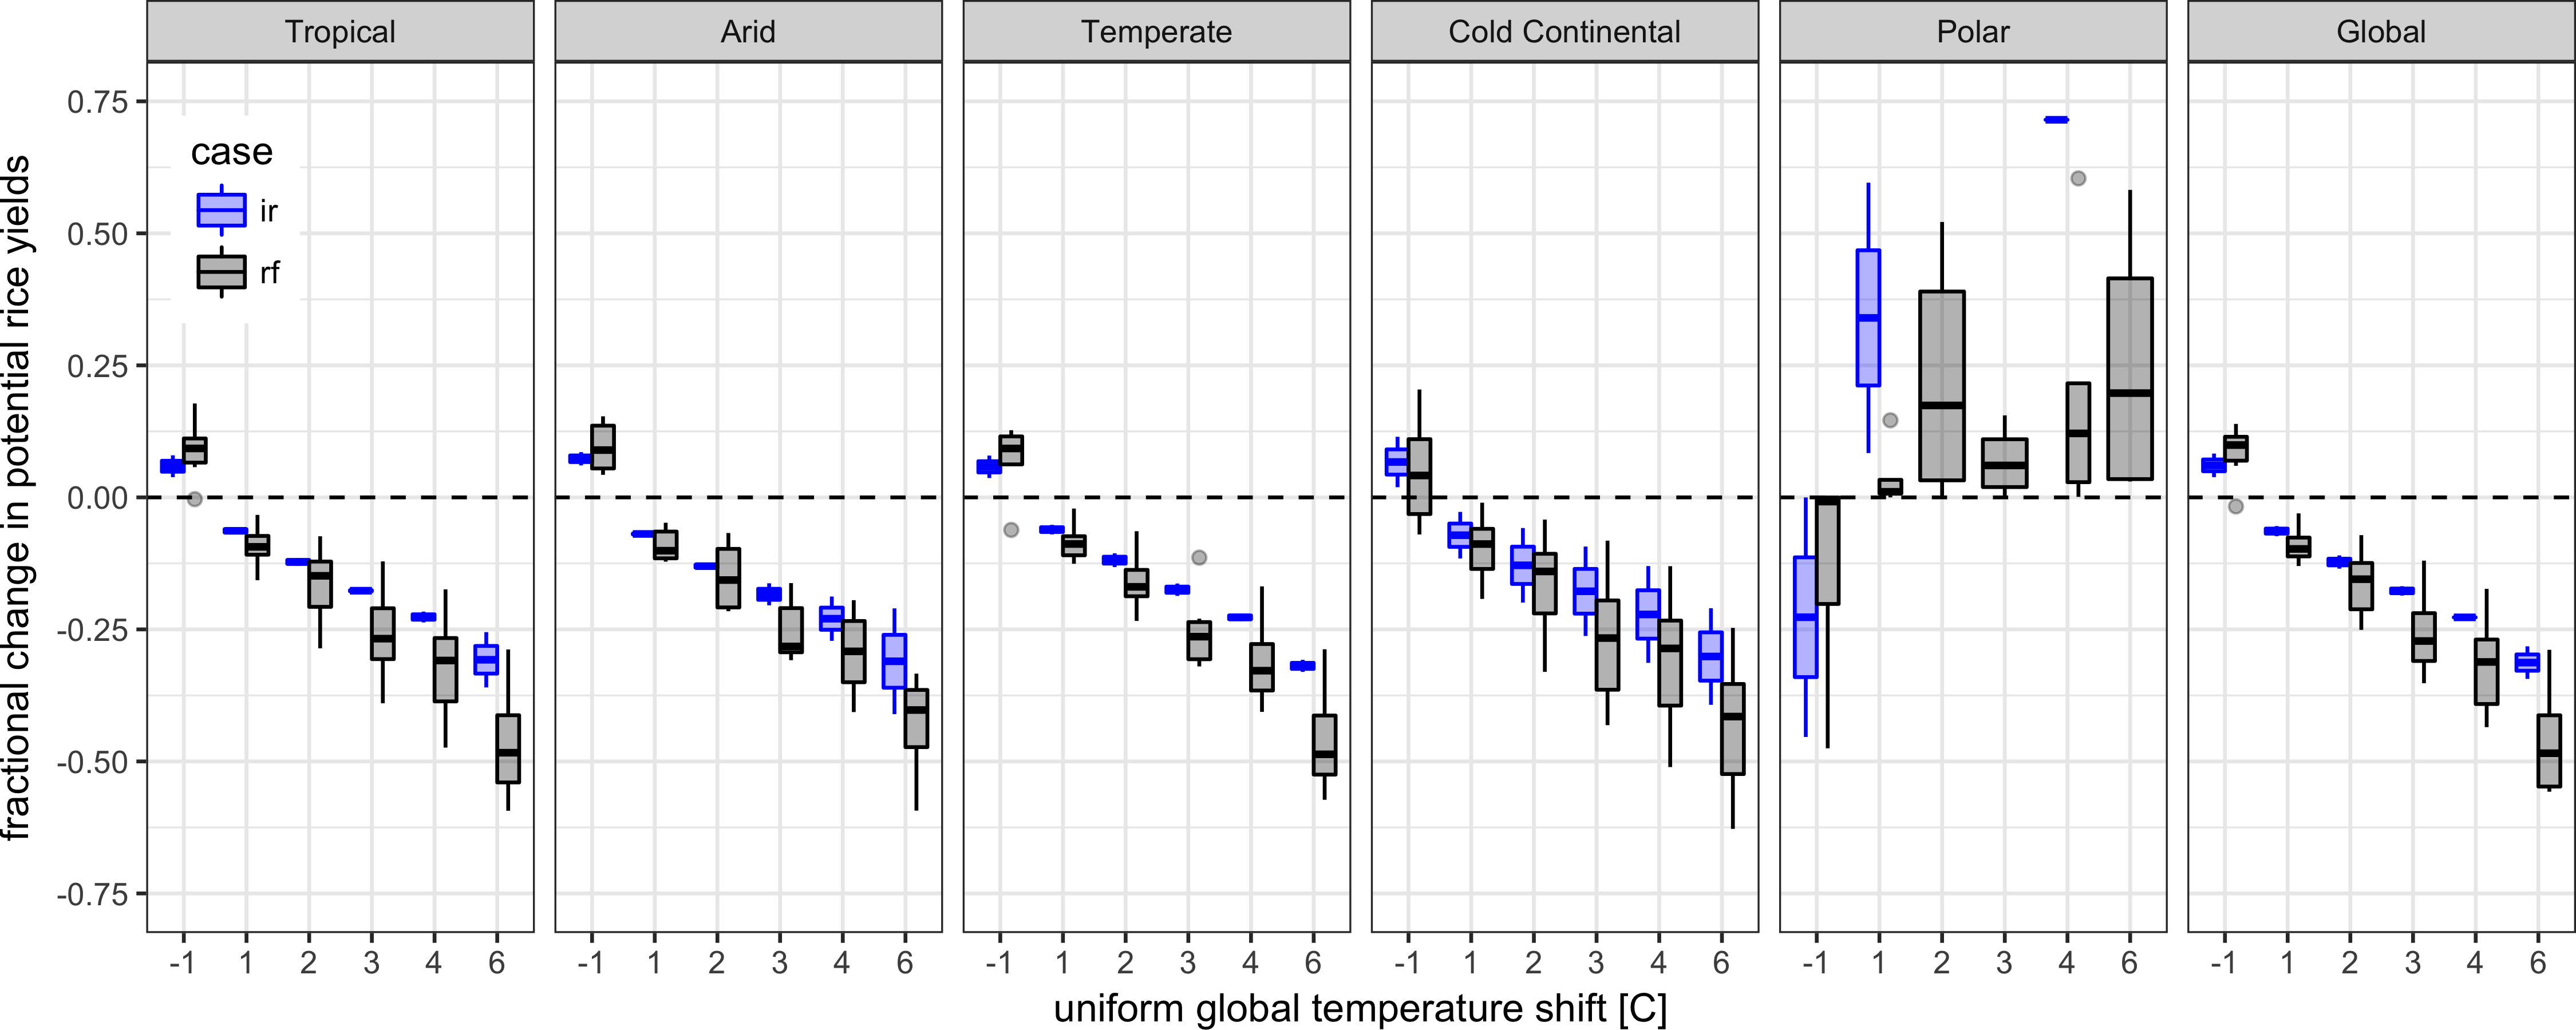
\includegraphics[width=\textwidth]{s_rice_sim_CG.png}\\
\caption{Rice simulation results. As in Figure 2 in the main text except comparing rainfed to irrigated rice across all grid cells. All other figure conventions match Figure 2 in the main text.}
\label{fig:maizeCG}
\end{figure}

\subsection{Currently cultivated area}
\begin{figure}[h!]
%S12
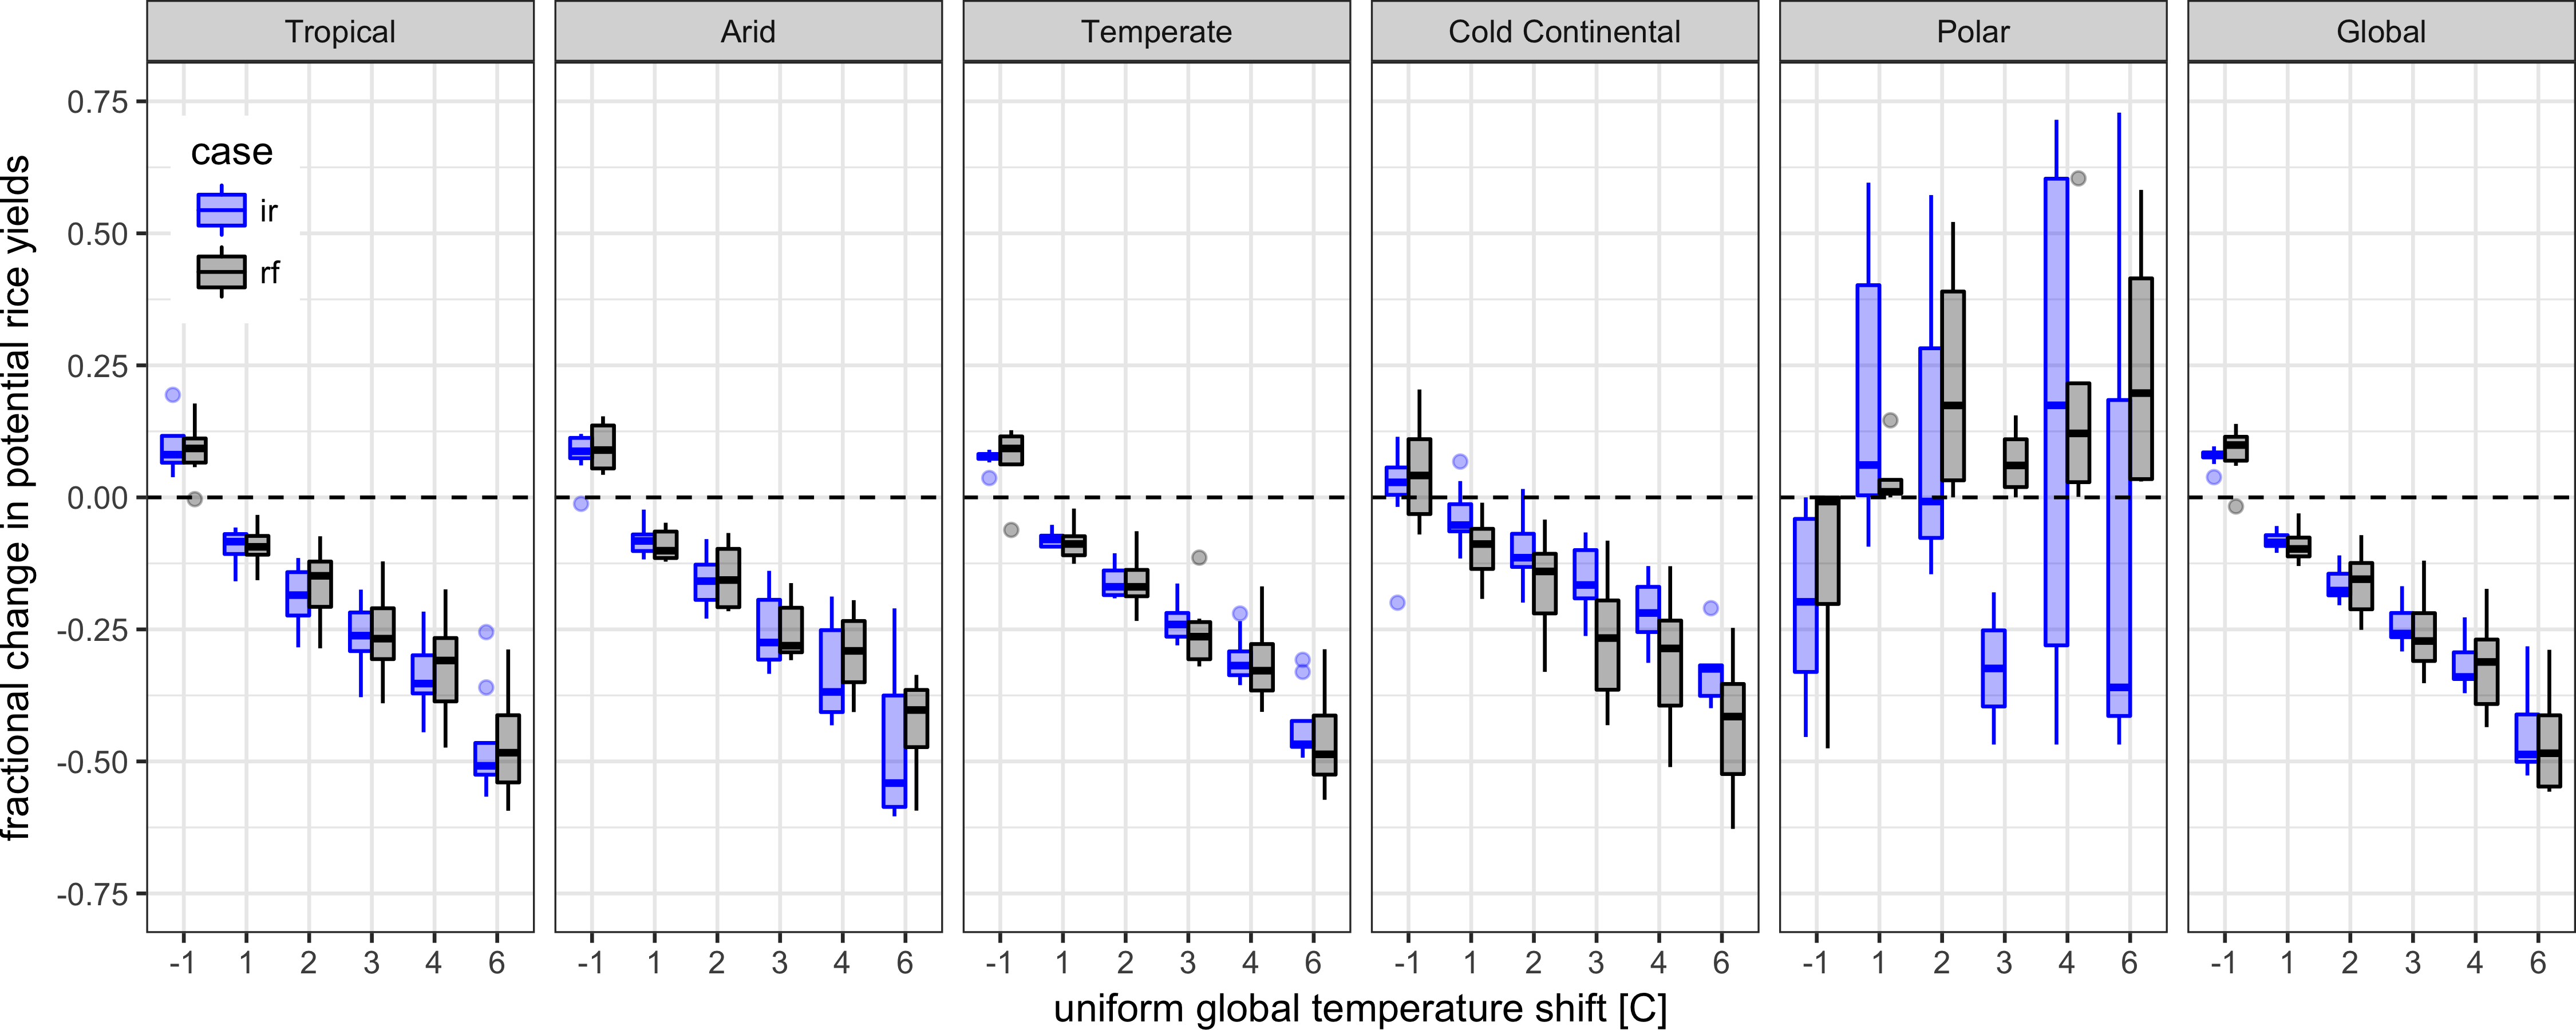
\includegraphics[width=\textwidth]{s_rice_sim_CG_area_weight.png}\\
\caption{Rice simulation results. As in Figure 2 in the main text except comparing rainfed to irrigated rice across currently cultivated hectares. All other figure conventions match Figure 2 in the main text.}
\label{fig:maizeCG}
\end{figure}

\clearpage
\section{Winter Wheat Simulations}
\subsection{All grid cells}
\begin{figure}[h!]
%S13
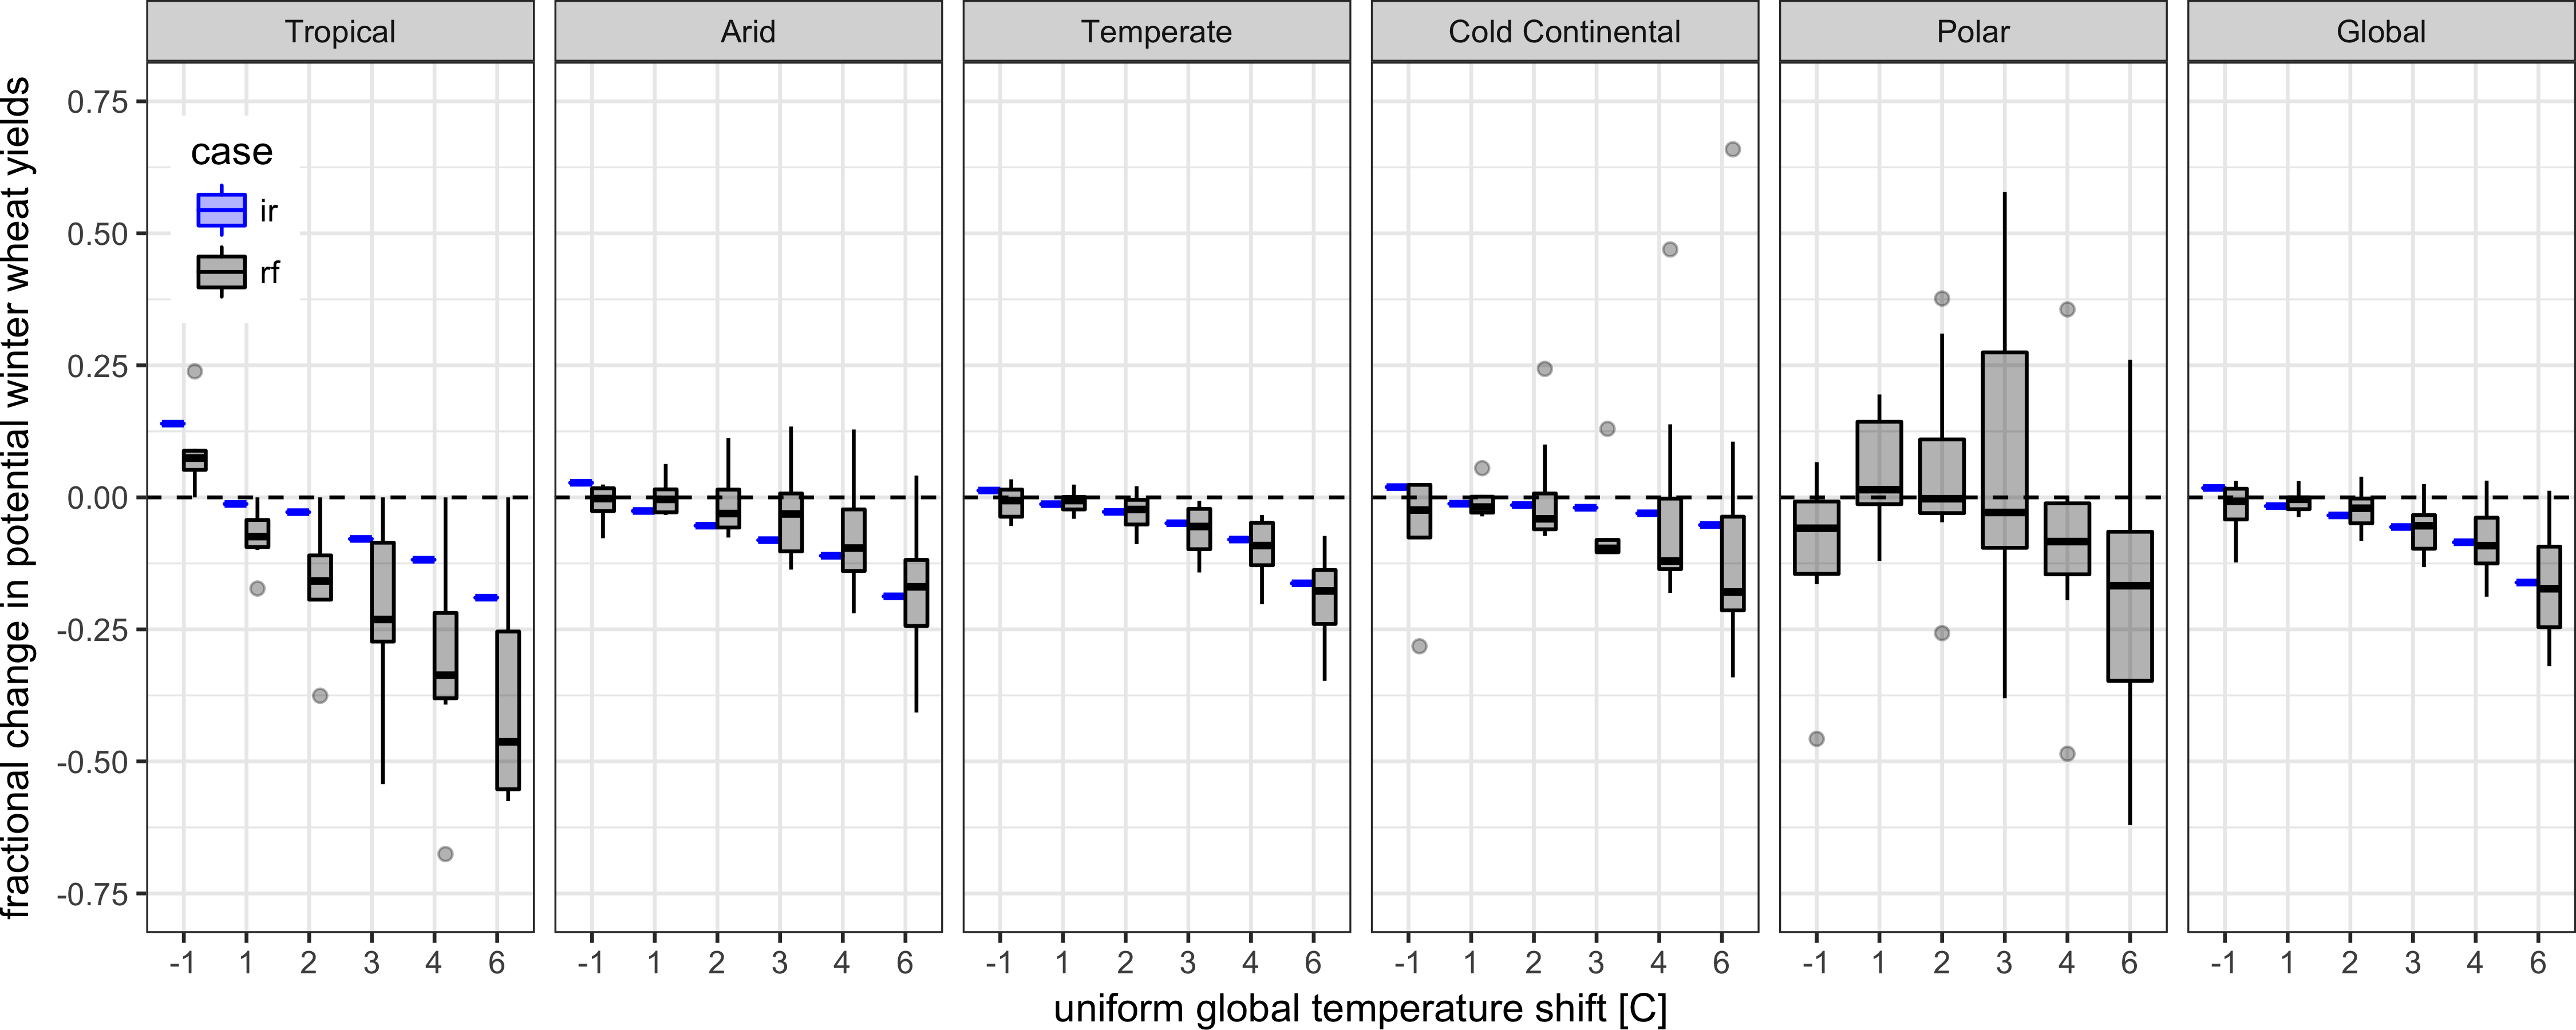
\includegraphics[width=\textwidth]{s_winter_wheat_sim_CG.png}\\
\caption{Winter wheat simulation results. As in Figure 2 in the main text except comparing rainfed to irrigated winter wheat across all grid cells. All other figure conventions match Figure 2 in the main text.}
\label{fig:maizeCG}
\end{figure}

\subsection{Currently cultivated area}
\begin{figure}[h!]
%S14
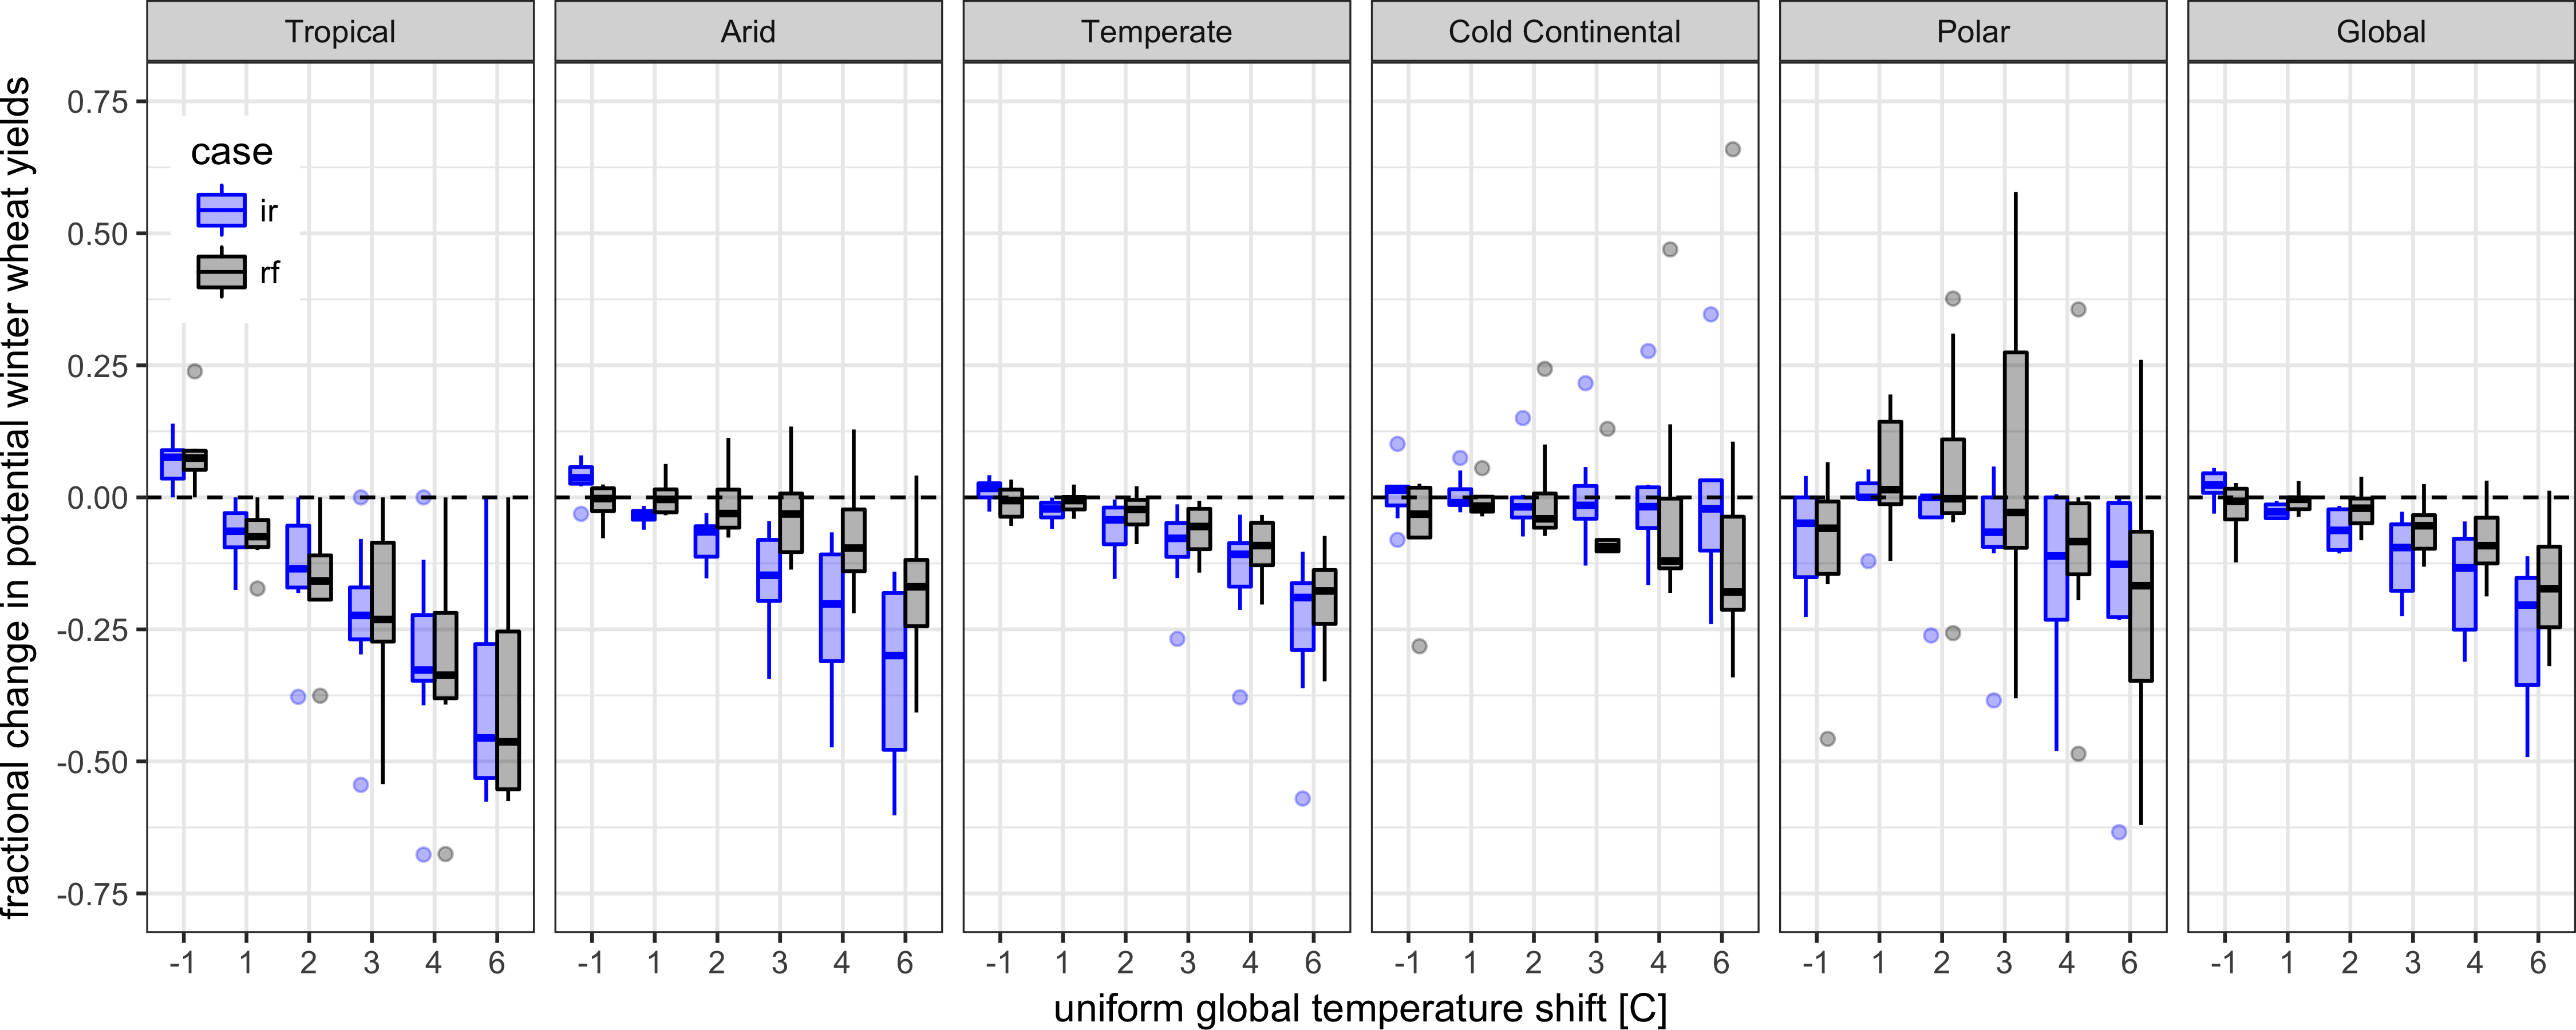
\includegraphics[width=\textwidth]{s_winter_wheat_sim_CG_area_weight.png}\\
\caption{Winter wheat simulation results. As in Figure 2 in the main text except comparing rainfed to irrigated winter wheat across currently cultivated hectares. All other figure conventions match Figure 2 in the main text.}
\label{fig:maizeCG}
\end{figure}

\clearpage
\section{Spring Wheat Simulations}
\subsection{All grid cells}
\begin{figure}[h!]
%S15
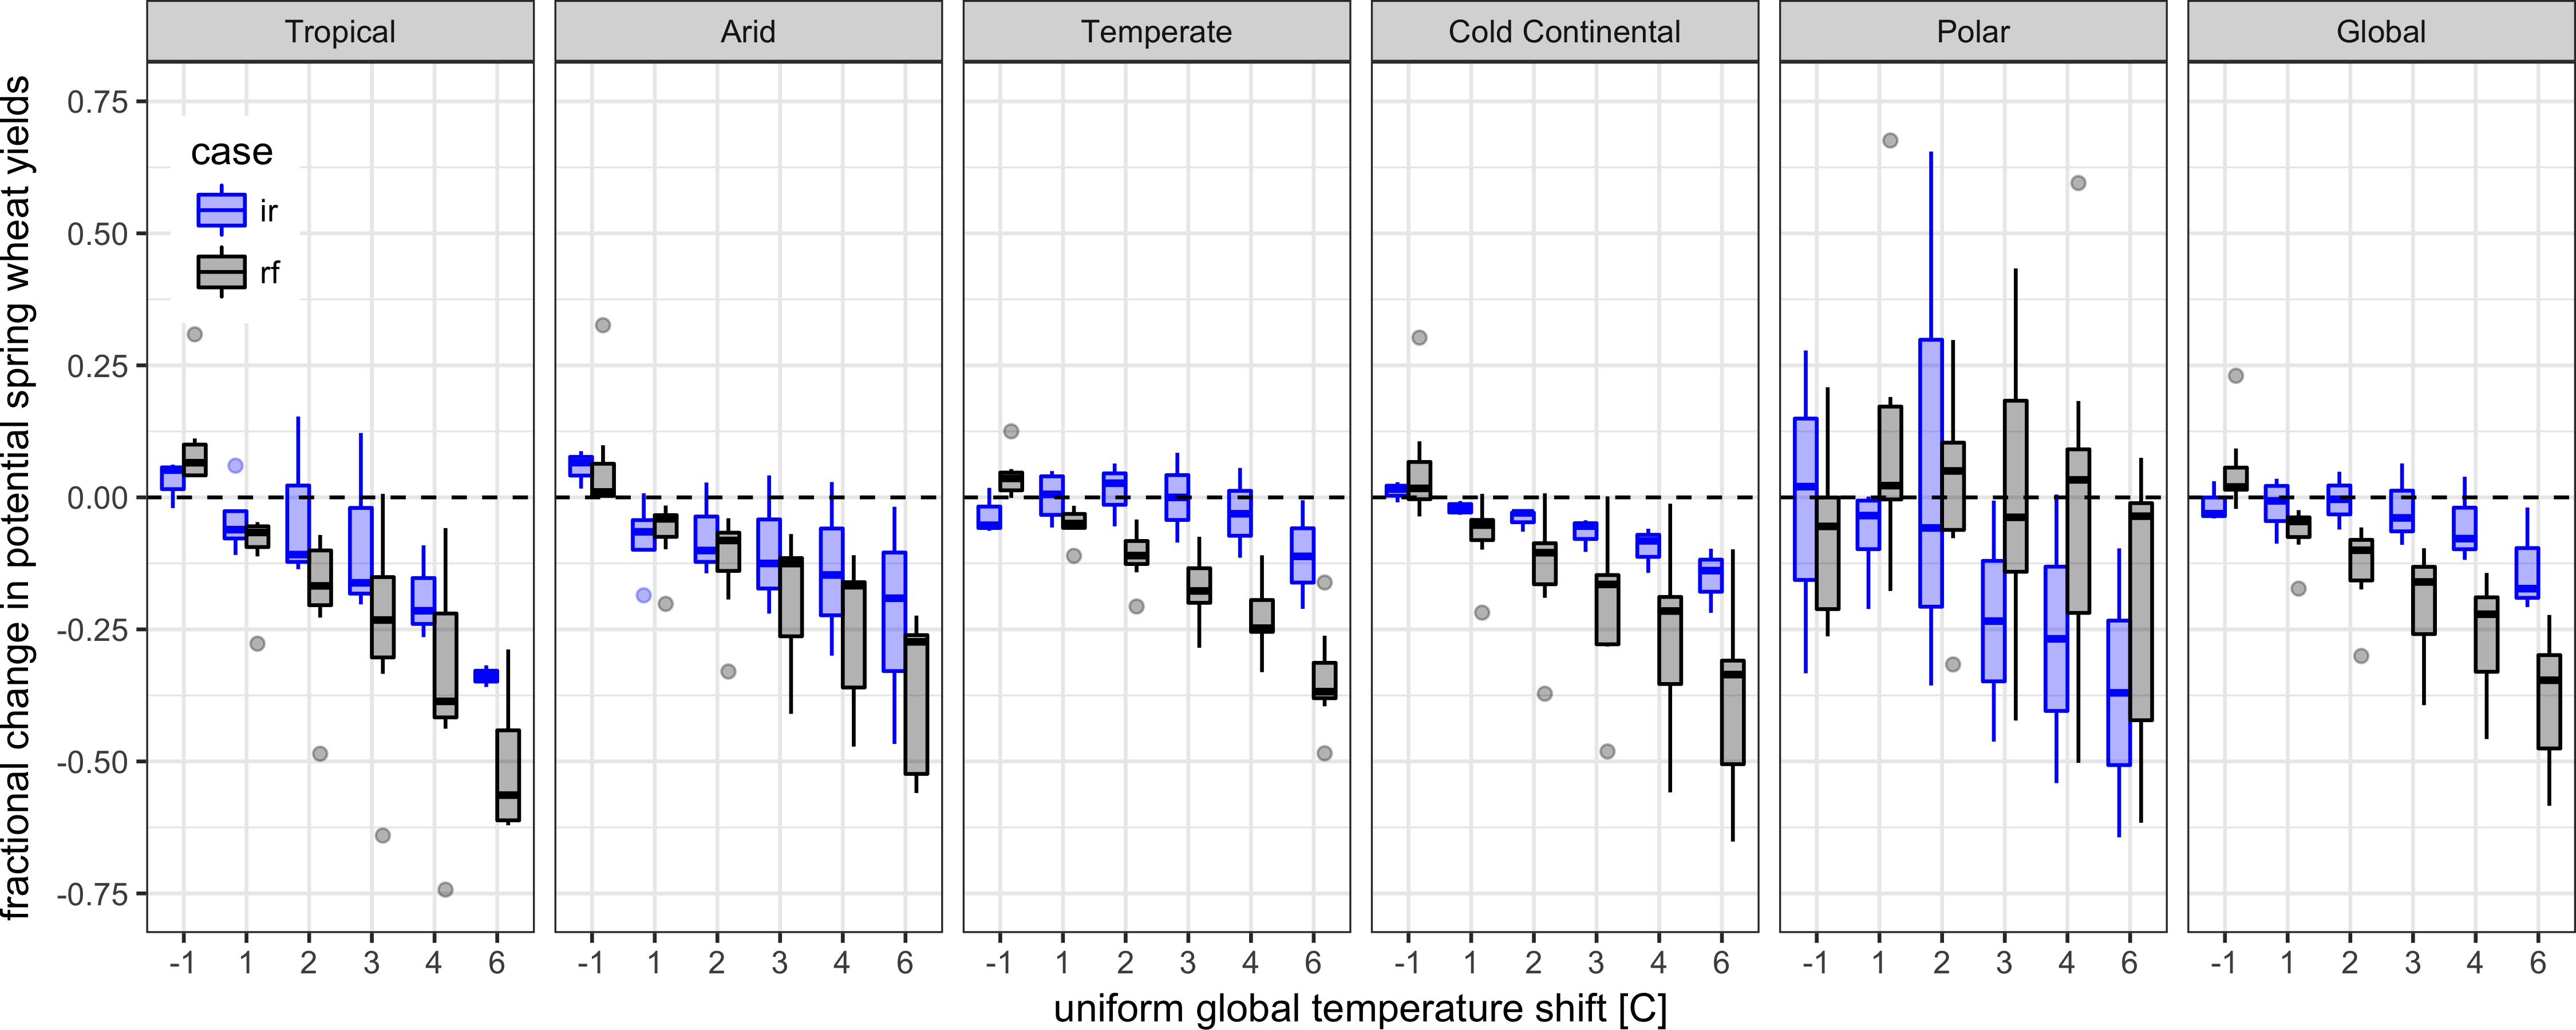
\includegraphics[width=\textwidth]{s_spring_wheat_sim_CG.png}\\
\caption{Spring wheat simulation results. As in Figure 2 in the main text except comparing rainfed to irrigated spring wheat across all grid cells. All other figure conventions match Figure 2 in the main text.}
\label{fig:maizeCG}
\end{figure}

\subsection{Currently cultivated area}
\begin{figure}[h!]
%S16
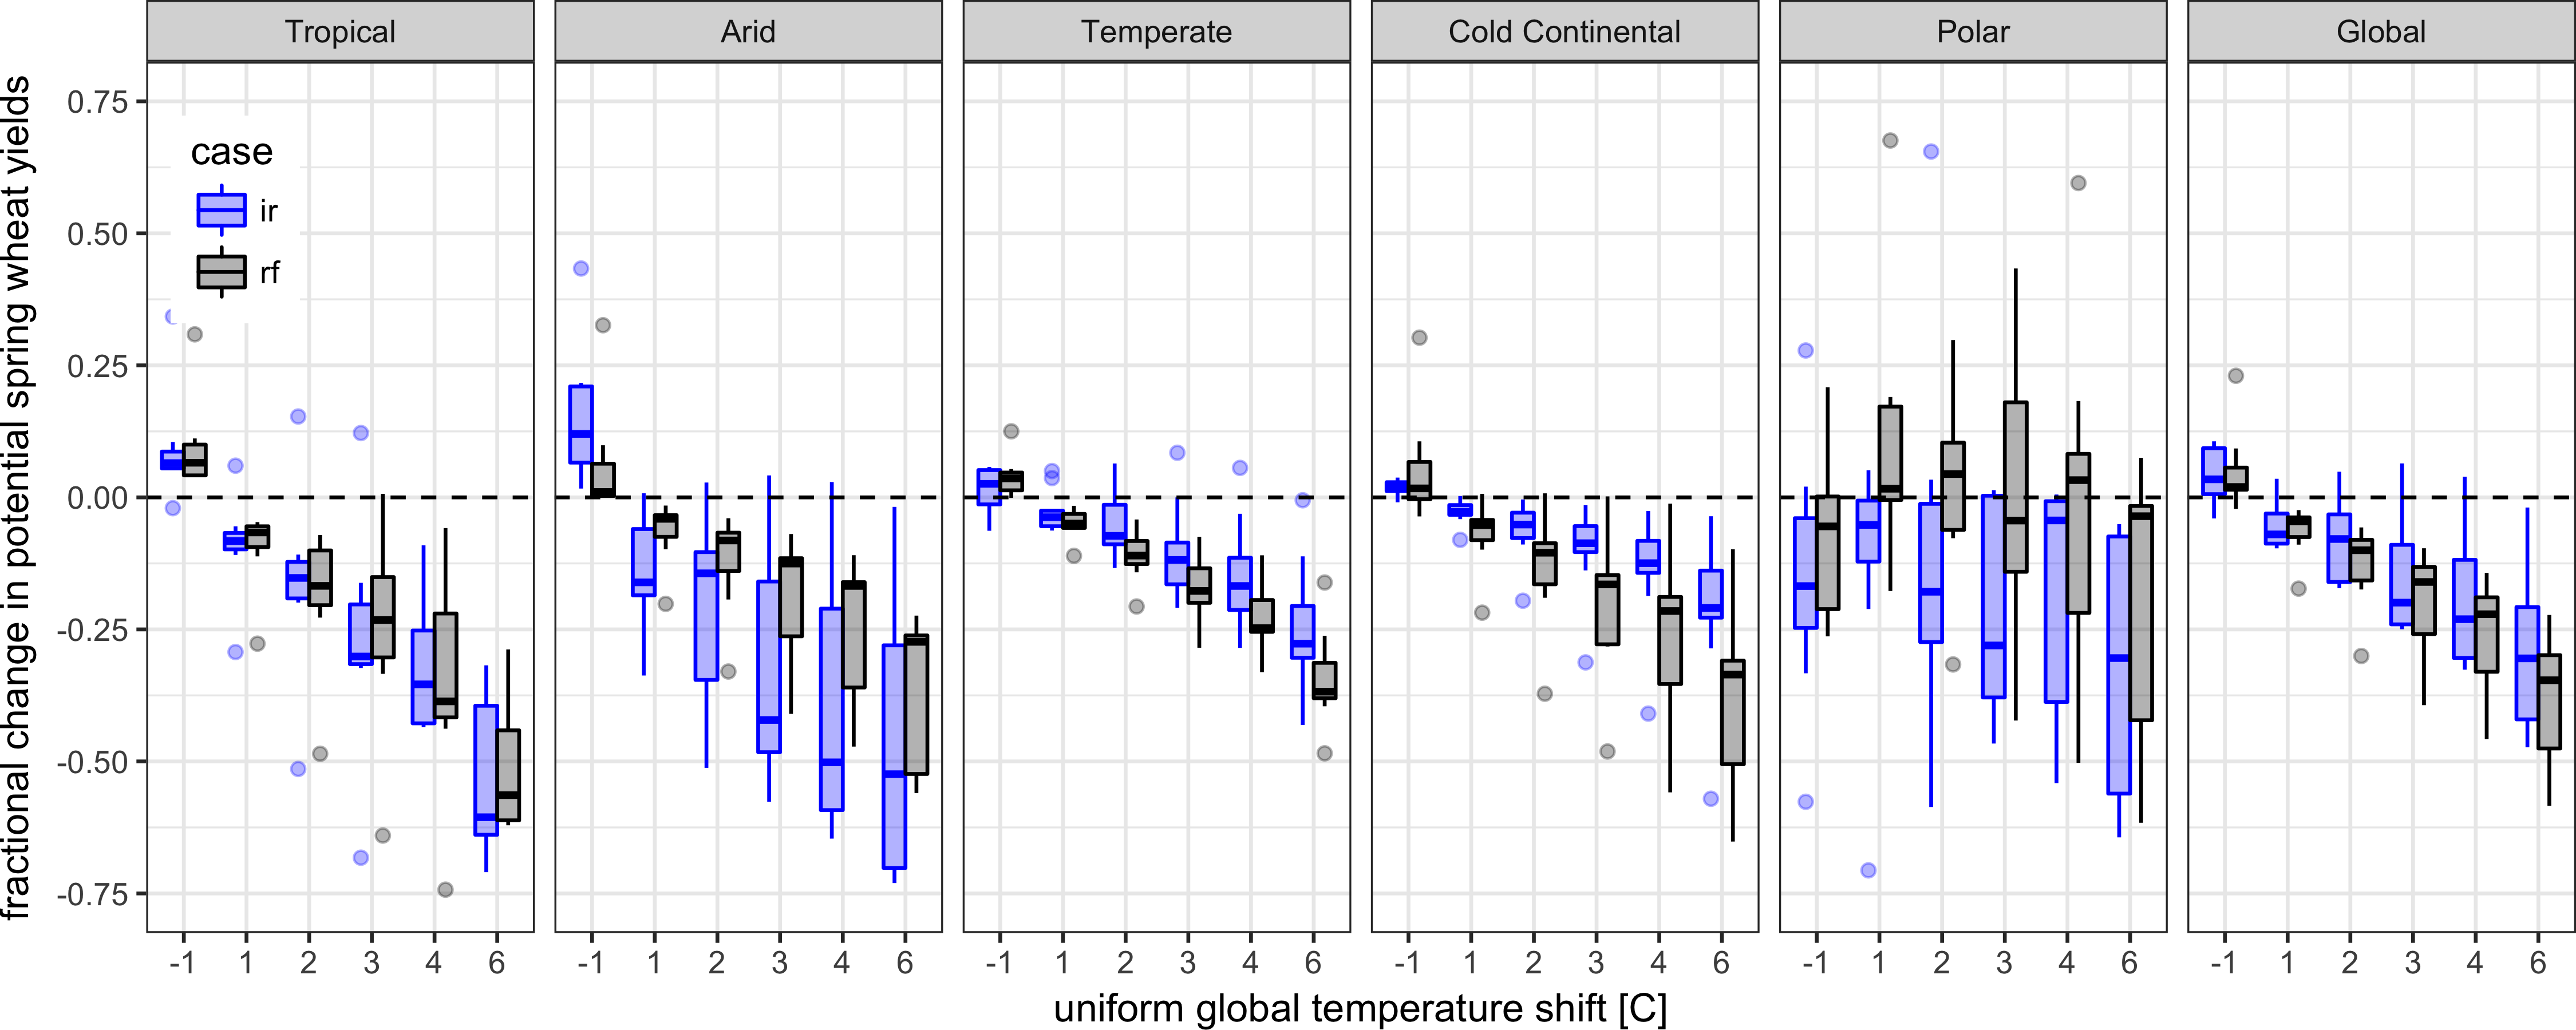
\includegraphics[width=\textwidth]{s_spring_wheat_sim_CG_area_weight.png}\\
\caption{Spring wheat simulation results. As in Figure 2 in the main text except comparing rainfed to irrigated spring wheat across currently cultivated hectares. All other figure conventions match Figure 2 in the main text.}
\label{fig:maizeCG}
\end{figure}


\clearpage 
\section{Wheat Simulations}
\begin{figure}[h!]
%S6
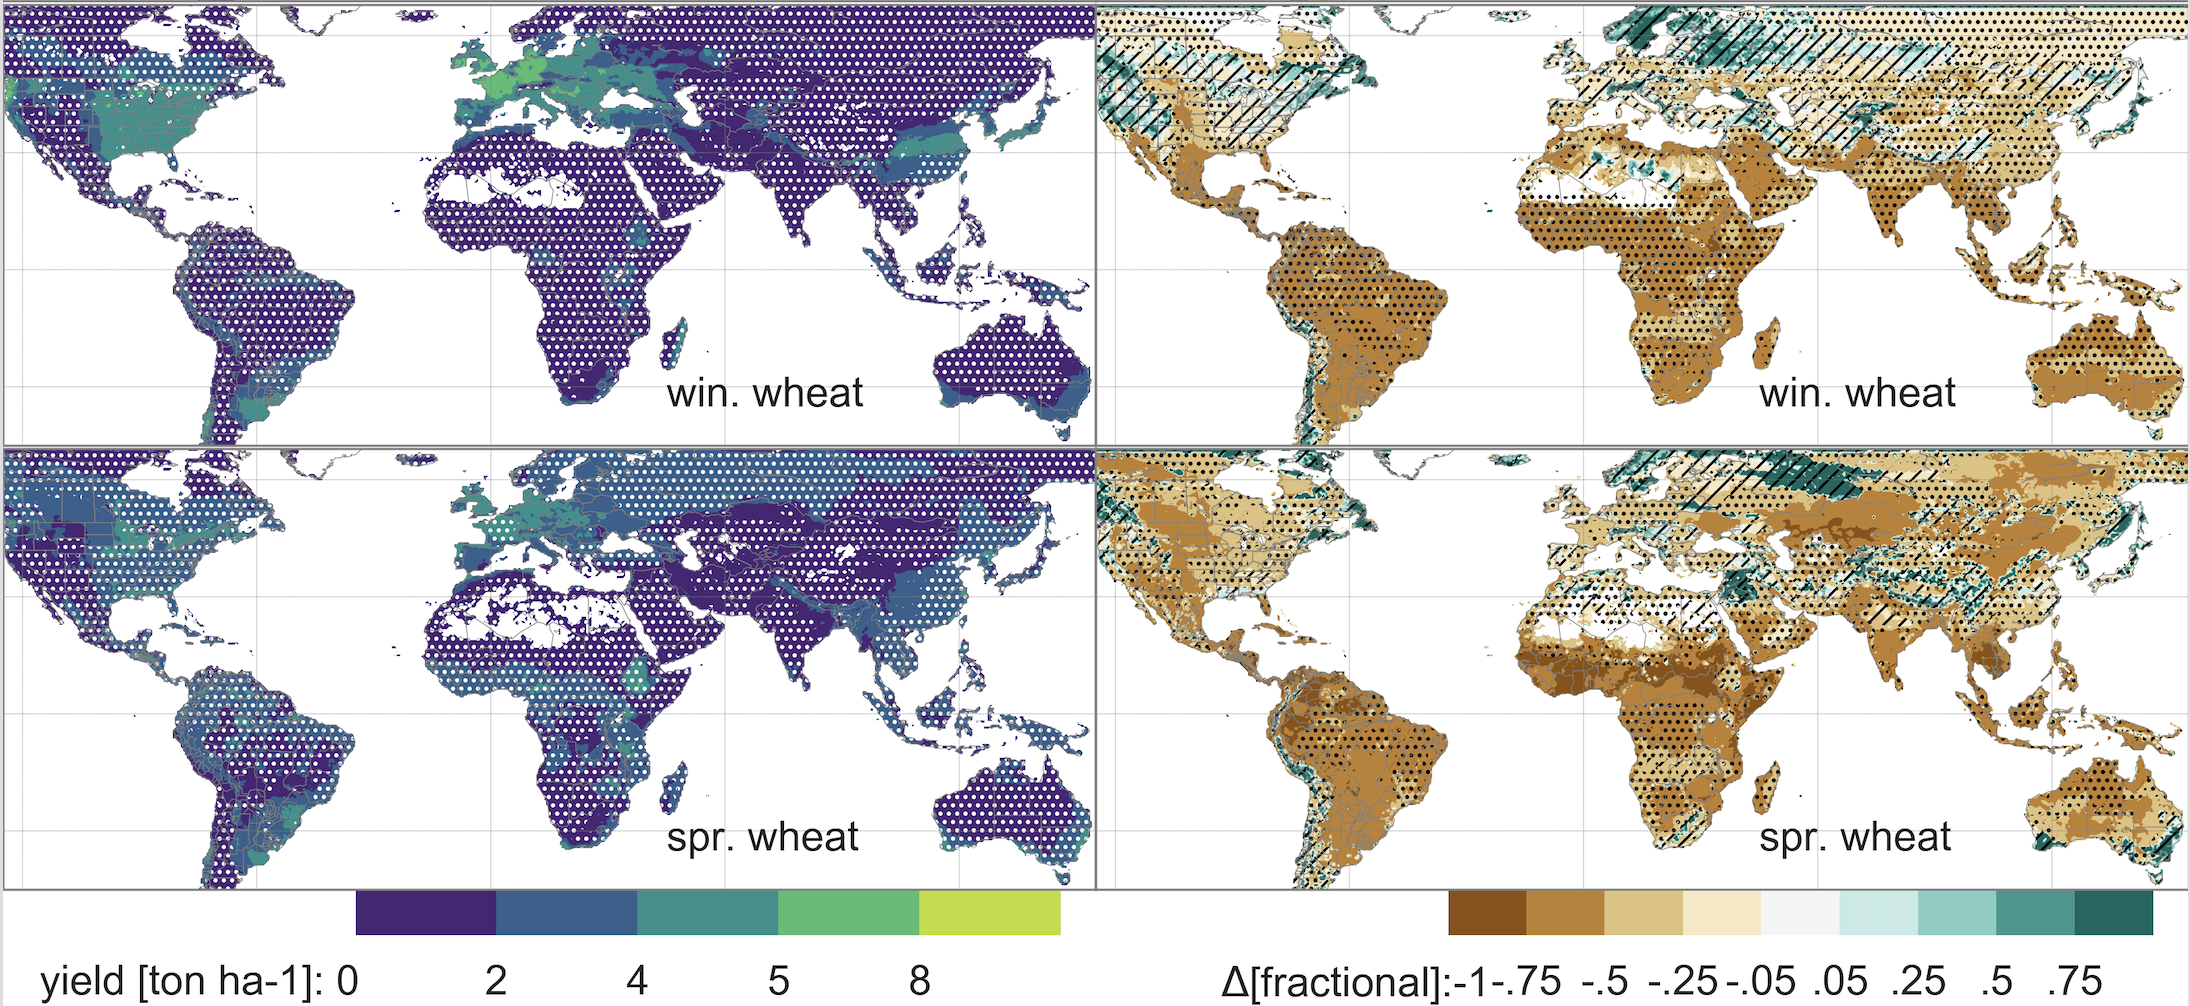
\includegraphics[width=\textwidth]{s_wheat_baseline.png}\\
\caption{Illustration of the spatial pattern of potential yields and potential yield changes in the GGCMI Phase II ensemble, for wheat. All figure conventions follow Figure 3 in the main text. Wheat model results in cold areas, where yield impacts are on average positive, also have the highest uncertainty. Wheat is also somewhat exceptional in that  also less impact in temperature and arid regions. The more complicated phenological development of winter wheat when compared to other crops is a potential source of the higher level of model disagreement.}
\label{fig:wheatbaseline}
\end{figure}